\documentclass[../../main.tex]{subfiles}
\begin{document}
\chapter{Background Work}

In this chapter, we delve into the foundational research areas central to this thesis. We begin by exploring avatars, examining various methods for their representation and animation. Following this, we review the evolution of Sign Language descriptions, tracing their progression from linear glosses to non-linear representations. Finally, we focus on the recent advancements in Sign Language synthesis, discussing various techniques and their implications for the field.

\section{Avatars}

Avatars are digital representations of characters or individuals, often used in virtual environments and simulations. They can be designed to resemble humans, animals, or fantastical beings, and are crucial in fields such as gaming, virtual reality, and digital communication. Avatars serve as a medium for interaction, allowing users to express themselves and engage with others in a digital space. 

\subsection{Skeleton}

The skeleton of a digital avatar is a crucial component for enabling realistic movement and animation. It consists of a hierarchical structure of bones, joints, and constraints that mimic the human skeletal system. This section explores several popular skeleton systems used in avatar creation and animation.

\subsubsection{Mixamo}

Mixamo is a widely used online platform that provides a vast library of pre-rigged 3D characters and animations. Developed by Adobe, Mixamo offers an easy-to-use interface where users can upload their 3D models and automatically rig them using Mixamo's auto-rigging tool. This tool identifies key points on the model and generates a skeleton with appropriate bone placements. Additionally, Mixamo offers a range of pre-made animations that can be applied to the rigged models, facilitating quick and efficient animation workflows. The platform supports various file formats and is compatible with many 3D software tools. A standard Mixamo skeleton consists of 65 bones, covering major body parts including the spine, arms, legs, hands, and head.

\begin{figure}
  \centering 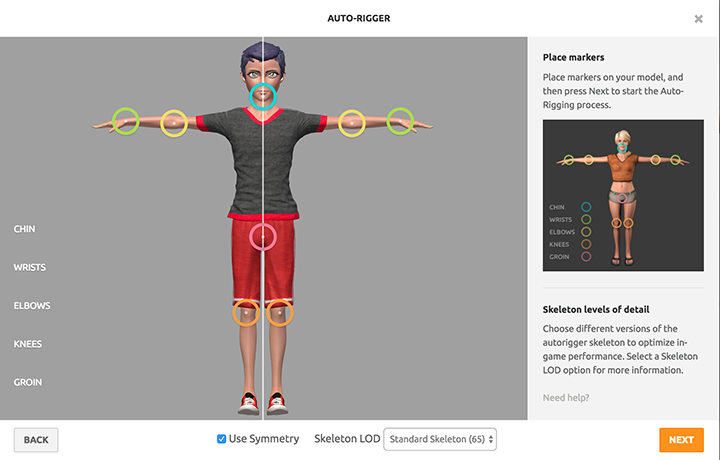
\includegraphics[width = 2.5in]{chapters/background_work/images/mixamo_autorigging.png}
  \caption{Autorigging using Mixamo}
  \label{fig:mixamo_autorigging}
\end{figure}

\begin{figure}
  \centering 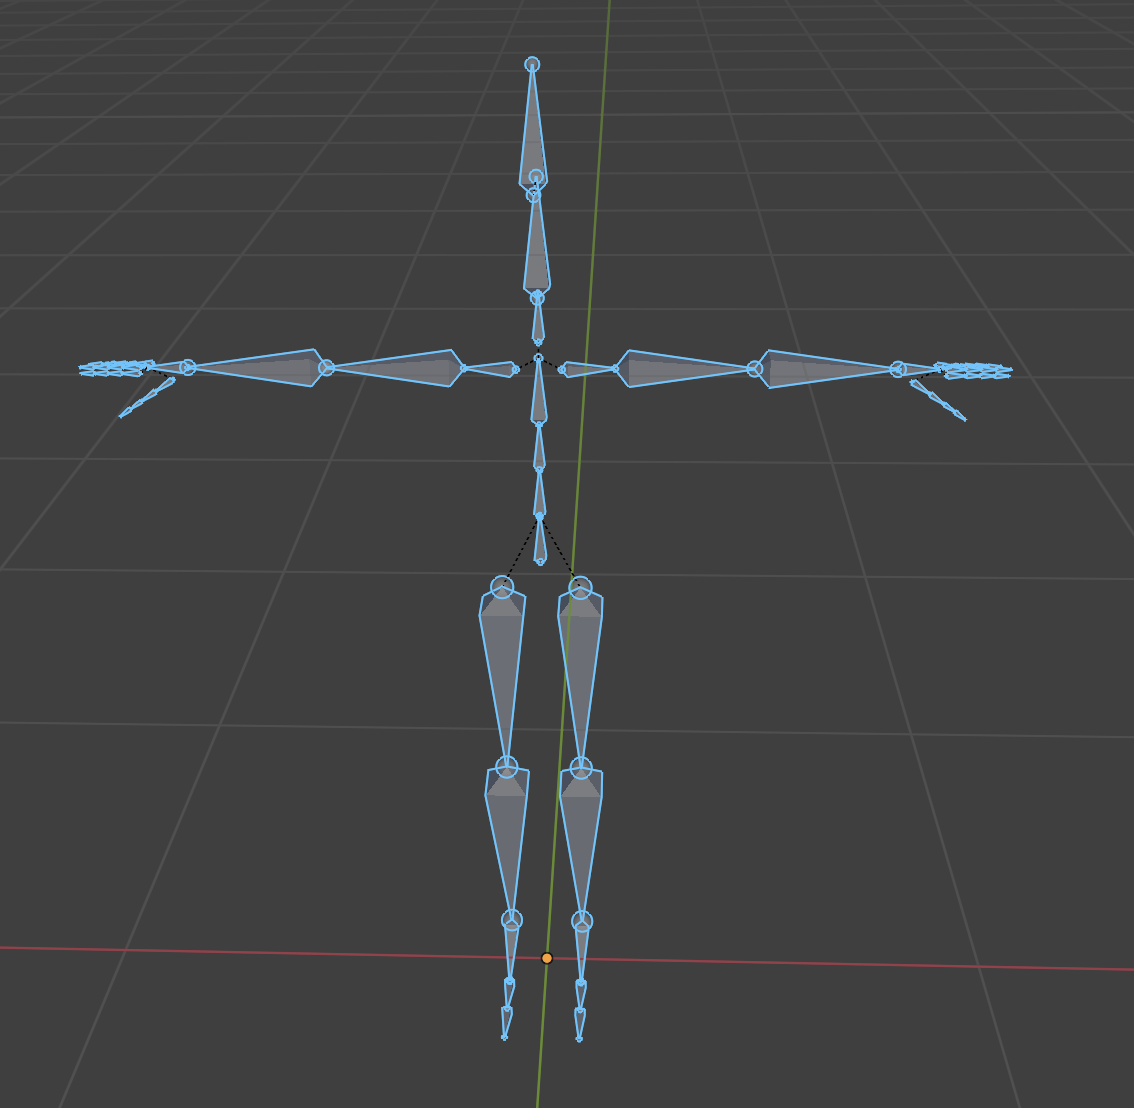
\includegraphics[width = 2.5in]{chapters/background_work/images/mixamo_skeleton.png}
  \caption{Standard Mixamo skeleton structure}
  \label{fig:mixamo_skeleton}
\end{figure}

\subsubsection{CMU}

The Carnegie Mellon University (CMU) Motion Capture Database is one of the most extensive collections of motion capture data available for public use. This database contains thousands of motion capture sequences recorded from real human performers, capturing a wide variety of movements and actions. The heirarchy of a CMU skeleton is shown in figure \ref{fig:cmu_skeleton}.

\begin{figure}
  \centering 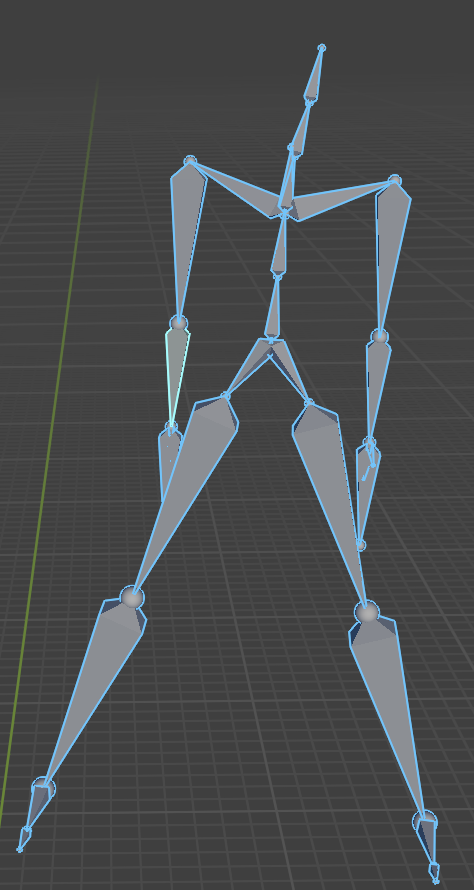
\includegraphics[width = 2.5in]{chapters/background_work/images/cmu_skeleton.png}
  \caption{CMU skeleton structure}
  \label{fig:cmu_skeleton}
\end{figure}

\subsubsection{Rigify}

Rigify is an add-on integrated in Blender. Rigify simplifies the process of rigging by providing a set of predefined rig templates that can be easily customized and applied to 3D models. The heirarchy of a Rigify skeleton is shown in figure \ref{fig:rigify_skeleton}.

\begin{figure}
  \centering 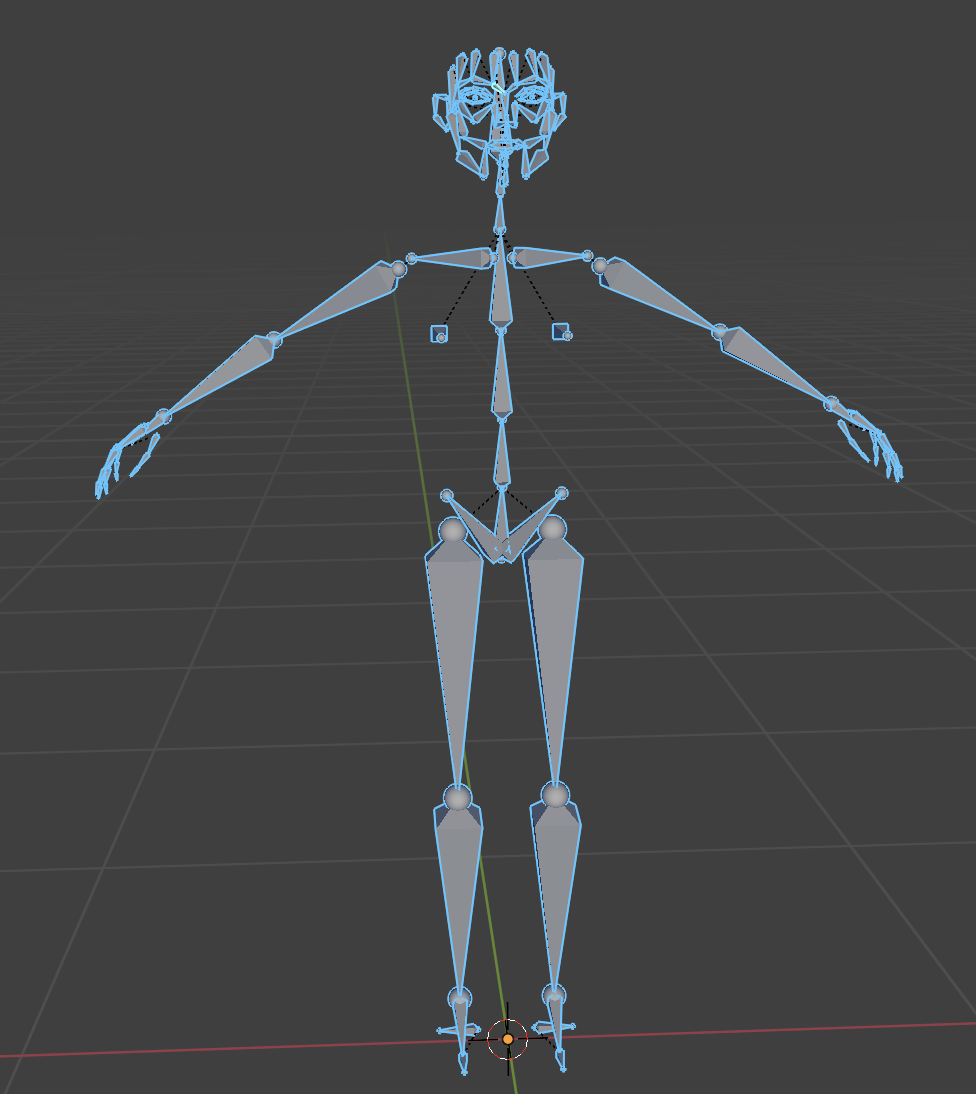
\includegraphics[width = 2.5in]{chapters/background_work/images/rigify_skeleton.png}
  \caption{Rigify skeleton}
  \label{fig:rigify_skeleton}
\end{figure}

\subsubsection{SMPL-X}

SMPL-X (Skinned Multi-Person Linear Model eXtended) is a state-of-the-art parametric model for generating highly detailed and anatomically accurate 3D human avatars. SMPL-X encodes the shape and pose of a character using a low-dimensional space, allowing for efficient representation and manipulation. Thus, a configuration of about 100 numbers can represent the pose as well as the shape of the avatar\ref{fig:latent_space_smplx}. The heirarchy of a SMPL-X skeleton is shown in figure \ref{fig:smpl_x_skeleton}.

\begin{figure}
  \centering 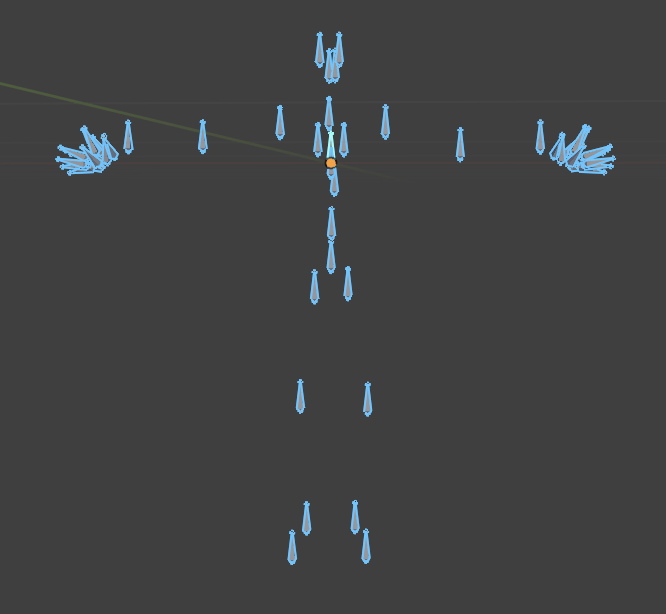
\includegraphics[width = 2.5in]{chapters/background_work/images/smpl_x_skeleton.png}
  \caption{SMPL-X skeleton}
  \label{fig:smpl_x_skeleton}
\end{figure}

\begin{figure}
  \centering 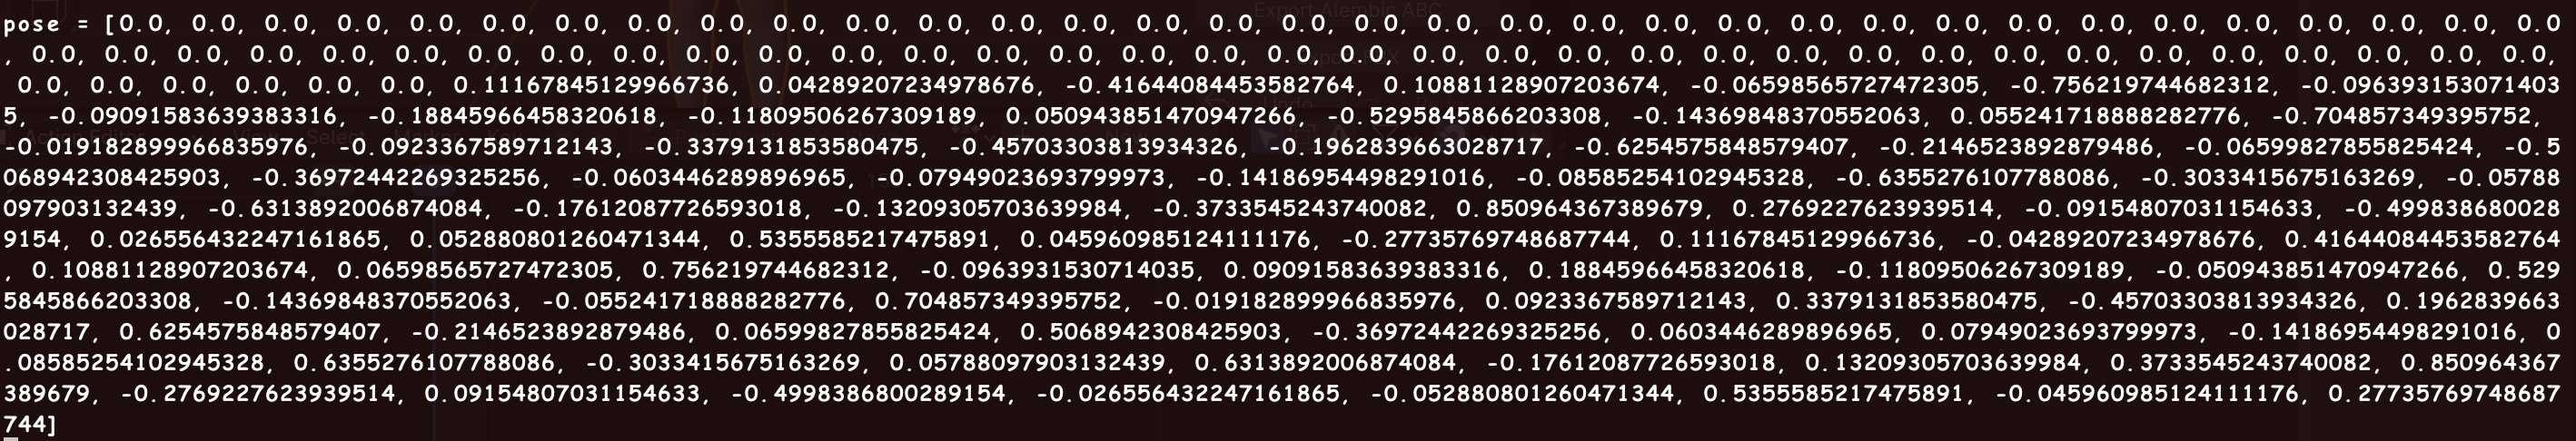
\includegraphics[width = 2.5in]{chapters/background_work/images/latent_space_smplx.png}
  \caption{SMPL-X latent space}
  \label{fig:latent_space_smplx}
\end{figure}

\subsection{Mesh}

The mesh of a digital avatar is the 3D model that forms the surface representation of the character. It consists of vertices, edges, and faces that define the shape and structure of the avatar. Creating and manipulating meshes is a fundamental aspect of 3D modeling and animation, allowing for detailed and realistic character designs.

\begin{figure}
  \centering 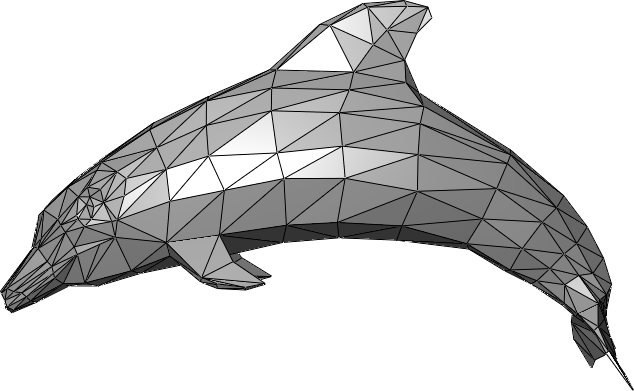
\includegraphics[width = 2.5in]{chapters/background_work/images/mesh.png}
  \caption{Mesh of a shark}
  \label{fig:mesh}
\end{figure}

\subsection{Texture}

Textures are 2D images applied to the surface of a 3D model to enhance its appearance and realism. Textures can represent various surface properties such as color, roughness, reflectivity, and transparency. Common types of textures include diffuse maps (color), specular maps (reflectivity), normal maps (surface detail), and roughness maps (surface smoothness). By combining different textures, artists can create visually compelling avatars with intricate surface details and lifelike appearances. These textures are often mapped onto the mesh of the avatar using UV mapping techniques to ensure proper alignment and scaling\ref{fig:texture_map}.

\begin{figure}
  \centering 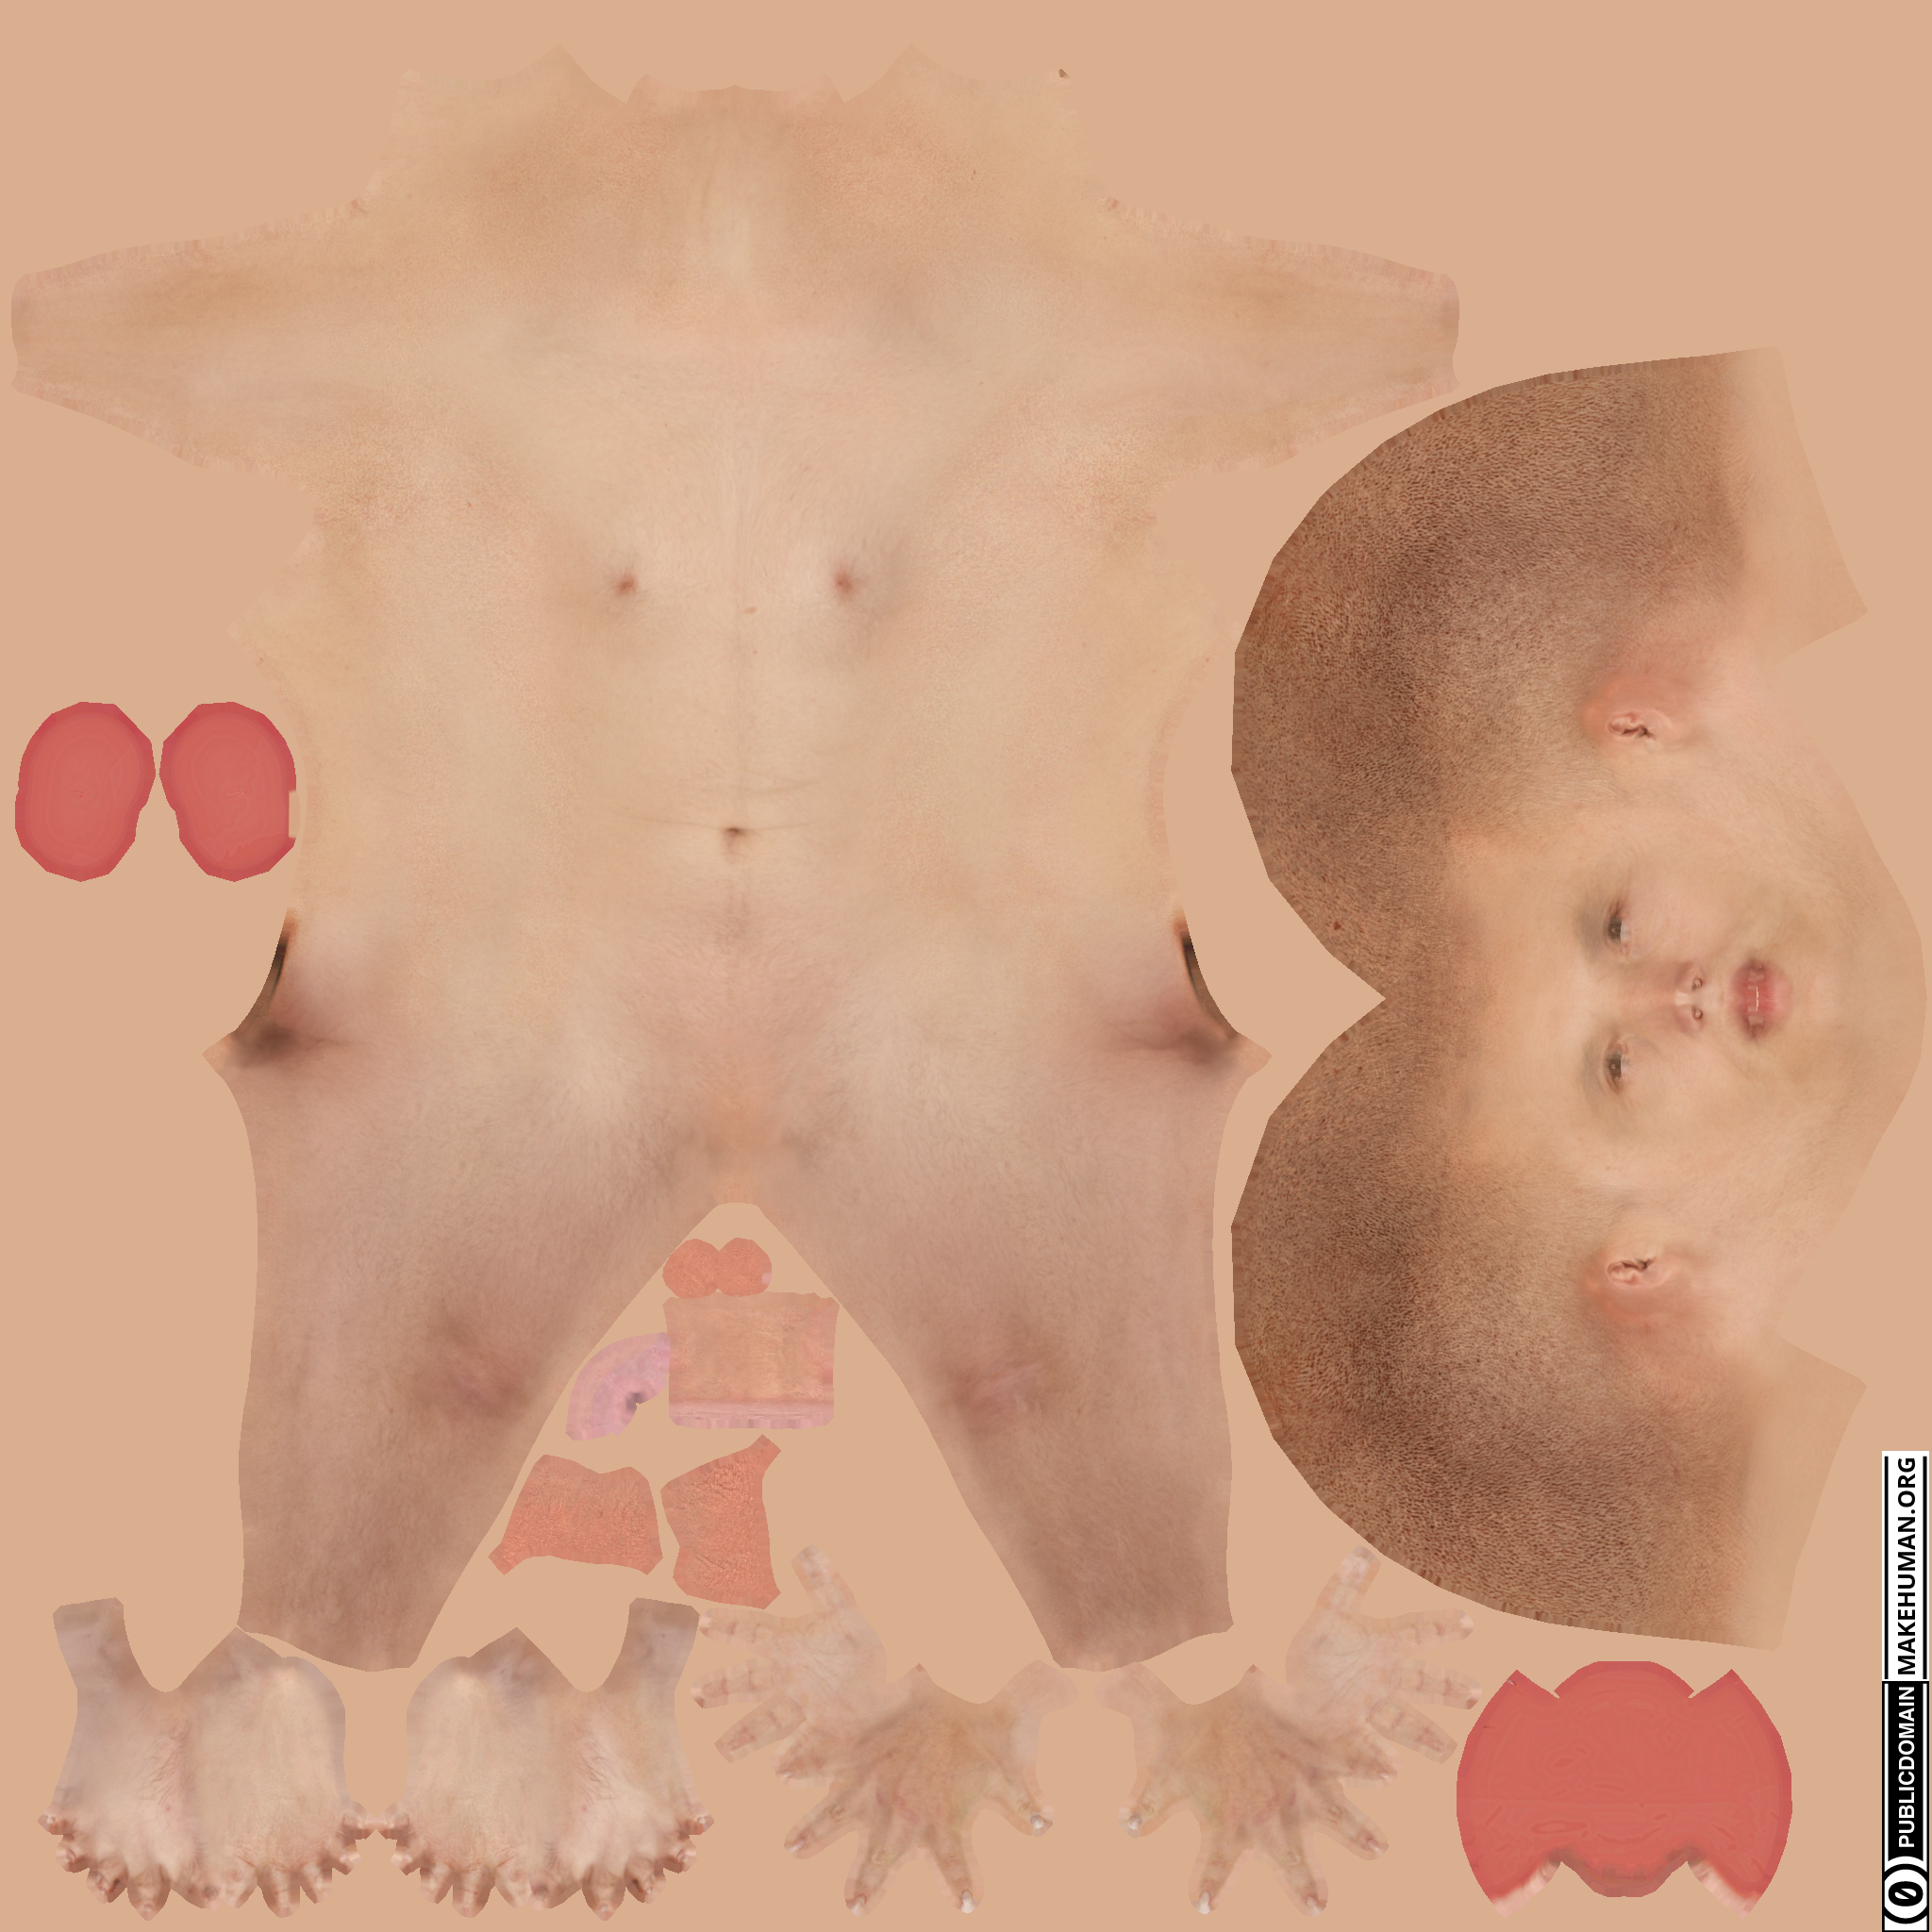
\includegraphics[width = 2.5in]{chapters/background_work/images/texture_map.png}
  \caption{Texture map of an avatar}
  \label{fig:texture_map}
\end{figure}

\subsubsection{Weight Painting}

Weight painting is a technique used to define how much influence each bone in a skeleton has over the surrounding mesh vertices. It plays a crucial role in ensuring that the mesh deforms naturally and realistically when the skeleton is animated. \ref{fig:weight_painting} shows an example of weight painting in Blender with the red color indicating high influence and blue indicating low influence.

\begin{figure}
  \centering 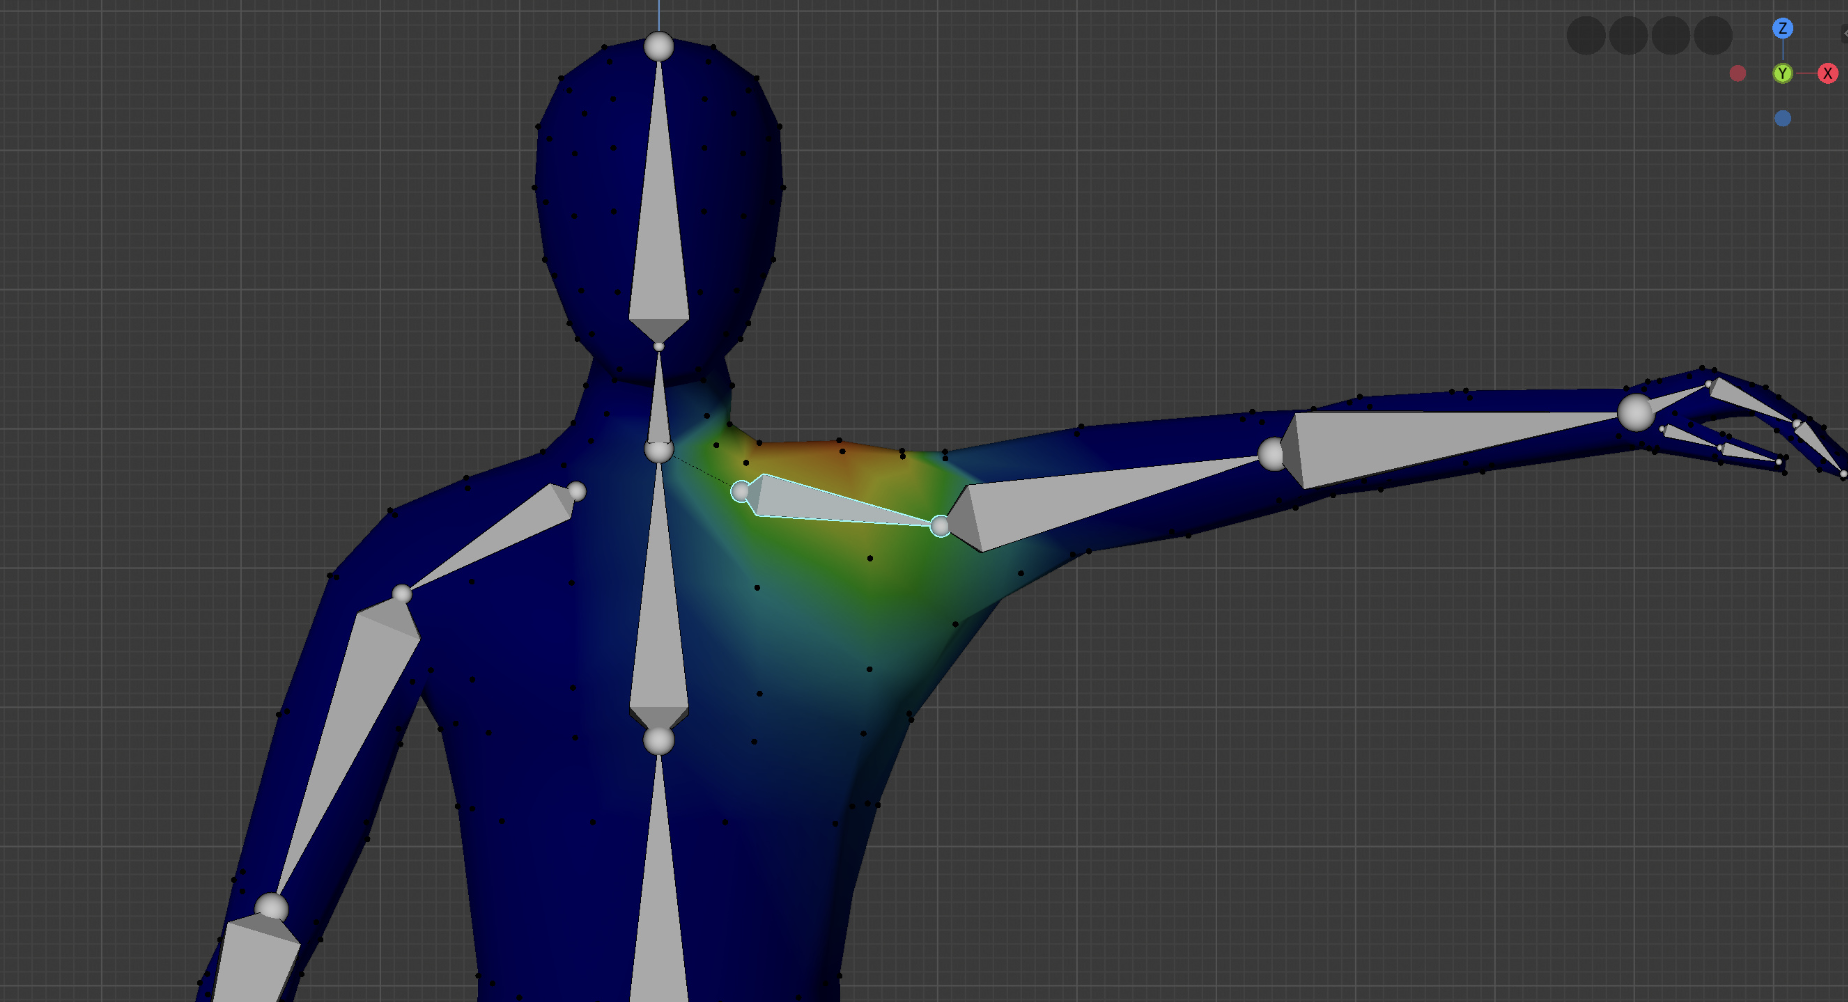
\includegraphics[width = 2.5in]{chapters/background_work/images/weight_painting.png}
  \caption{Weight painting}
  \label{fig:weight_painting}
\end{figure}

\subsubsection{Face}

Modeling and animating the face of an avatar is a complex task that involves creating detailed meshes and intricate animation controls to capture expressions and movements accurately. Blend shapes\ref{fig:blendshapes_example} are used to create different facial expressions by interpolating between multiple versions of a mesh. This technique allows animators to blend between various expressions smoothly, such as smiling, frowning, or blinking. Adding bones to the facial mesh allows for more granular control over facial movements\ref{fig:facial_bones}. Each bone can control different parts of the face, such as the jaw, eyebrows, and eyelids. This method is often used in conjunction with blend shapes to enhance expressiveness.

\begin{subfigure}{0.33\linewidth}
  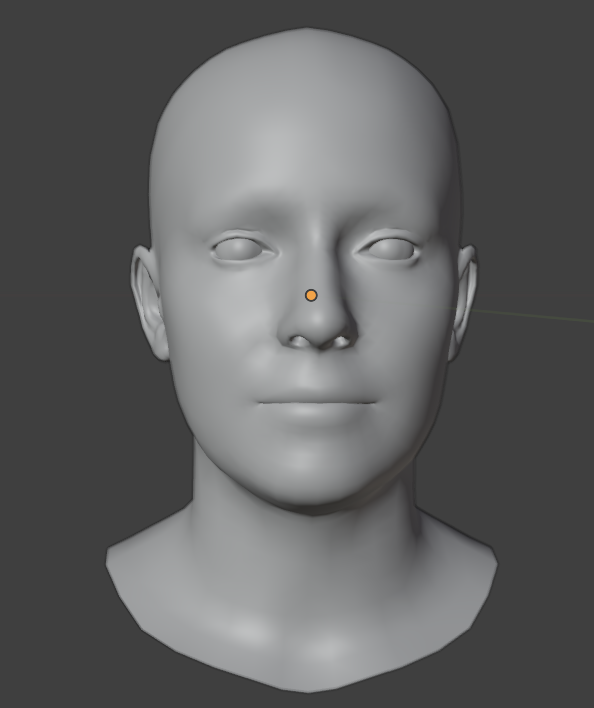
\includegraphics[width=\linewidth]{chapters/background_work/images/blendshapes_example/blendshapes_example_1.png}
  \caption{Blendshape smile at 0}
\end{subfigure}
\hfill
\begin{subfigure}{0.33\linewidth}
  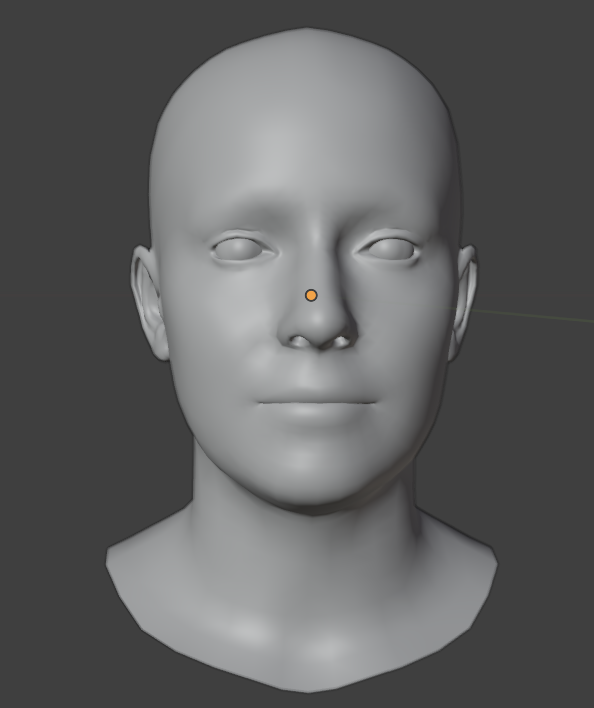
\includegraphics[width=\linewidth]{chapters/background_work/images/blendshapes_example/blendshapes_example_1.png}
  \caption{Blendshape smile at 0.5}
\end{subfigure}
\hfill
\begin{subfigure}{0.33\linewidth}
  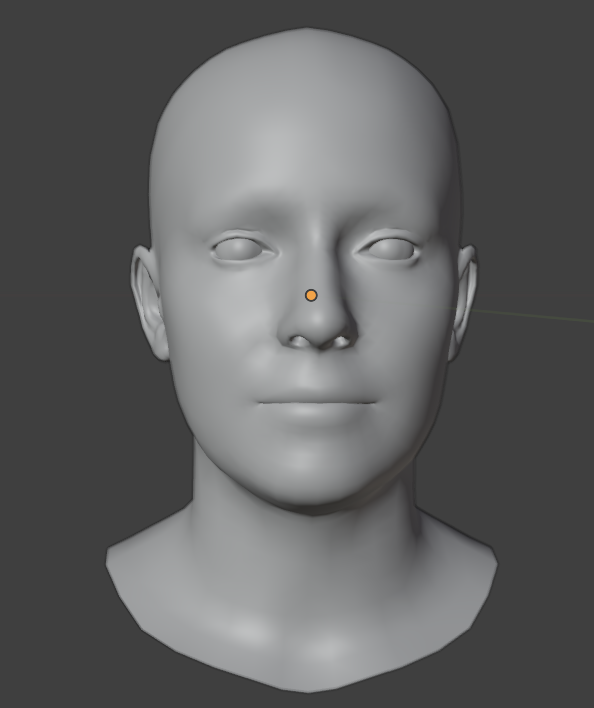
\includegraphics[width=\linewidth]{chapters/background_work/images/blendshapes_example/blendshapes_example_1.png}
  \caption{Blendshape smile at 1}
  \label{fig:blendshapes_example}
\end{subfigure}

\begin{figure}
  \centering 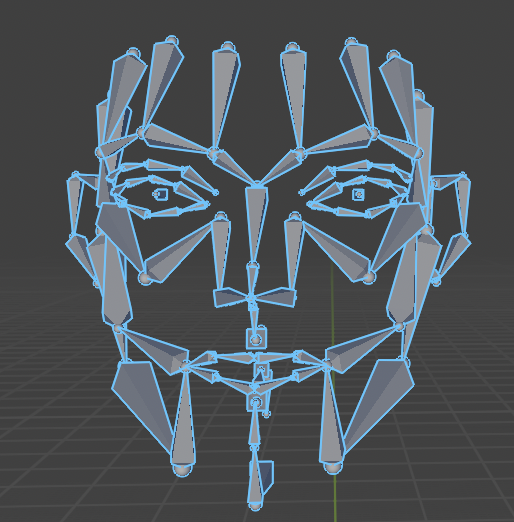
\includegraphics[width = 2.5in]{chapters/background_work/images/facial_bones.png}
  \caption{Facial bones for eyes, jaw and tongue}
  \label{fig:facial_bones}
\end{figure}

\subsubsection{Rig}

A rig is the final system used by the artists to animate the avatars. This is done by doing all the above systems in order i.e. creating a skeleton, mesh, texture, weight painting, facial blendshapes, implementing IK and FK systems, and adding constraints\ref{fig:rig_example}.

\begin{figure}
  \centering 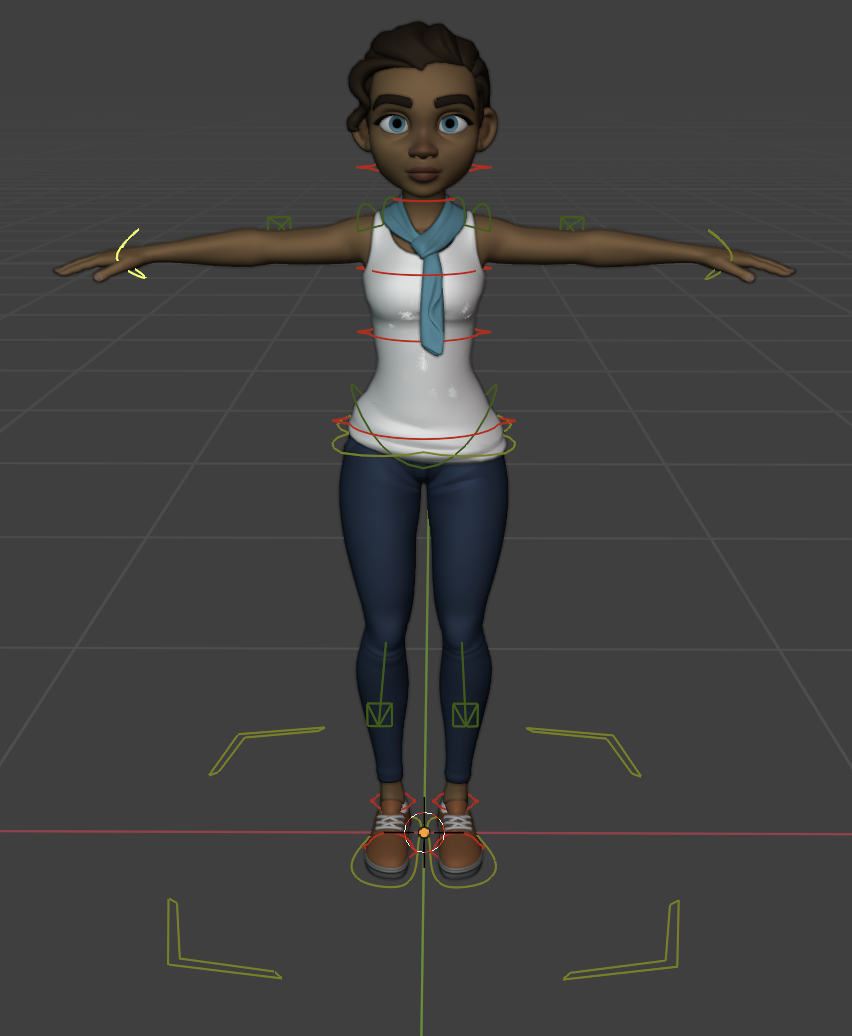
\includegraphics[width = 2.5in]{chapters/background_work/images/rig_example.png}
  \caption{Rain rig by Blender studio}
  \label{fig:rig_example}
\end{figure}

\subsection{Procedural Avatar Creation}

Procedural avatar creation involves the use of algorithms and software tools to automatically generate 3D characters with minimal manual intervention. This approach can significantly speed up the character creation process, allowing for the rapid development of detailed and diverse avatars. This section explores several prominent tools and models used for procedural avatar creation.

\subsubsection{MakeHuman}

MakeHuman is an open-source tool specifically designed for the rapid prototyping of humanoid avatars. It allows users to create 3D human models through an intuitive interface where parameters such as gender, age, ethnicity, and body proportions can be adjusted using sliders\ref{fig:makehuman_example}.

\begin{figure}
  \centering 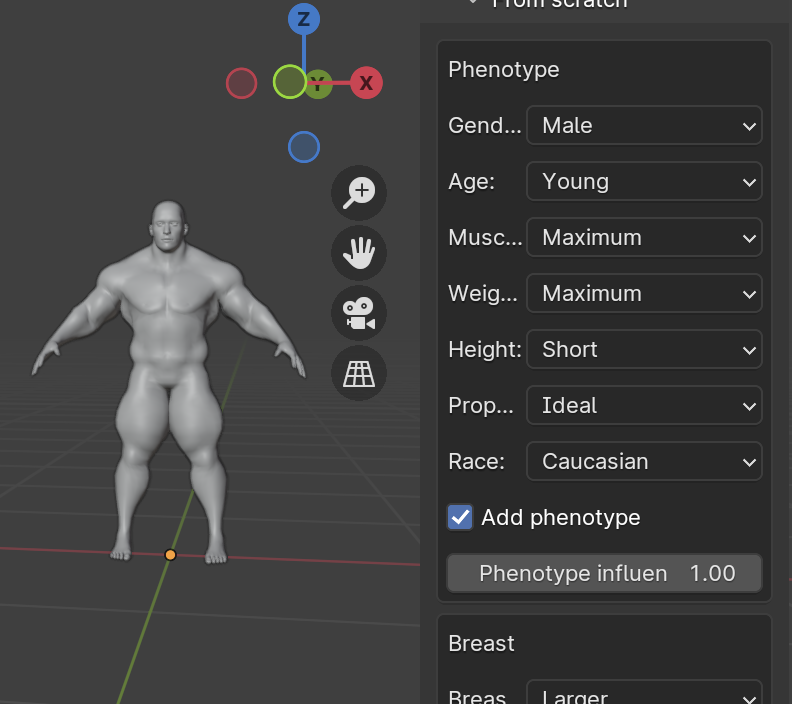
\includegraphics[width = 2.5in]{chapters/background_work/images/makehuman_example.png}
  \caption{Avatar creation using MakeHuman}
  \label{fig:makehuman_example}
\end{figure}

\subsubsection{SMPL-X or Meshcapade}

Just like MakeHuman, SMPL-X can create avatars with parameters suchs as weight, height, age, etc. However, SMPL-X can also be created using images of a person. This allows it to be more realistic than MakeHuman\ref{fig:smpl_creation_example}.

\begin{figure}
  \centering 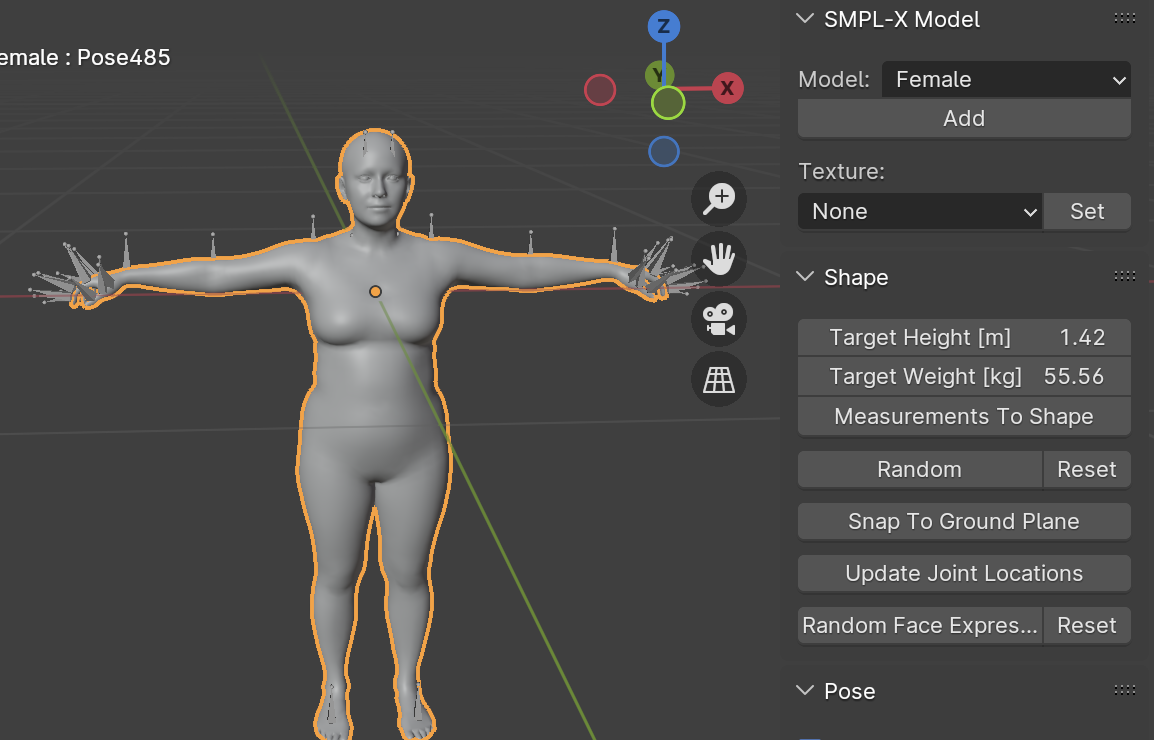
\includegraphics[width = 2.5in]{chapters/background_work/images/smpl_creation_example.png}
  \caption{SMPL-X avatar creation using Meshcapade}
  \label{fig:smpl_creation_example}
\end{figure}

\subsubsection{MetaHuman}

MetaHuman Creator, developed by Epic Games, is a tool for creating ultra-realistic digital humans. The tool's emphasis on realism and detail makes it a powerful resource for creating lifelike characters for games, films, and other interactive experiences\ref{fig:metahuman_example}. MetaHumans are the most realistic avatars available today, with high-quality textures, detailed facial expressions, and advanced animation controls.

\begin{figure}
  \centering 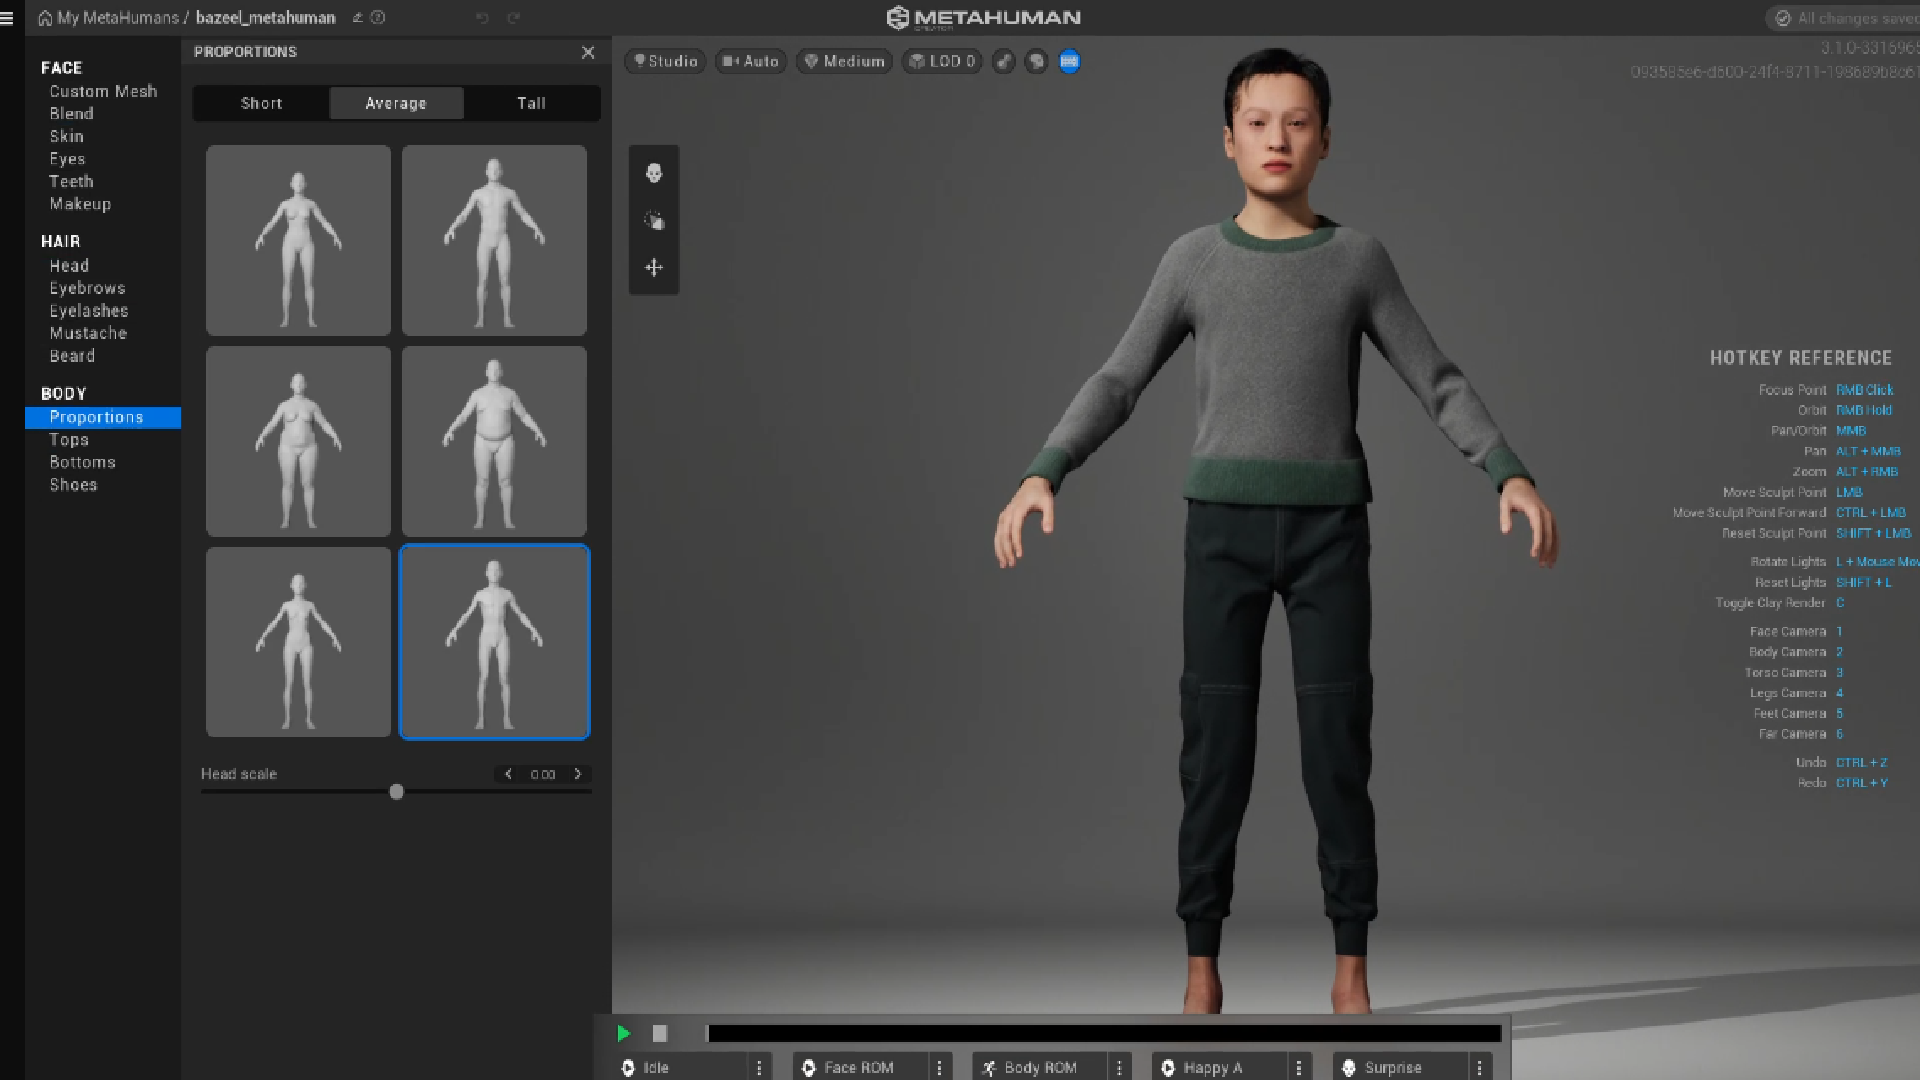
\includegraphics[width = 2.5in]{chapters/background_work/images/metahuman_example.png}
  \caption{Avatar creation using MetaHuman}
  \label{fig:metahuman_example}
\end{figure}

\subsection{Avatar Animation}

The methods used for animating avatars range from manual to automated processes, each offering unique benefits and challenges. This section explores the key methods used in avatar animation.

\subsubsection{Manual Keyframing}

Manual keyframing is a traditional animation technique where animators define specific poses, known as keyframes, at critical points in time. These keyframes mark the start and end points of any smooth transition or movement. The intermediate poses are then calculated using interpolation\ref{fig:keyframing}. This method provides animators with precise control over every aspect of the avatar’s movement, making it ideal for achieving nuanced and detailed animations. However, manual keyframing can be time-consuming and requires a high level of skill and expertise to ensure realistic and fluid motion.

\begin{figure}
  \centering 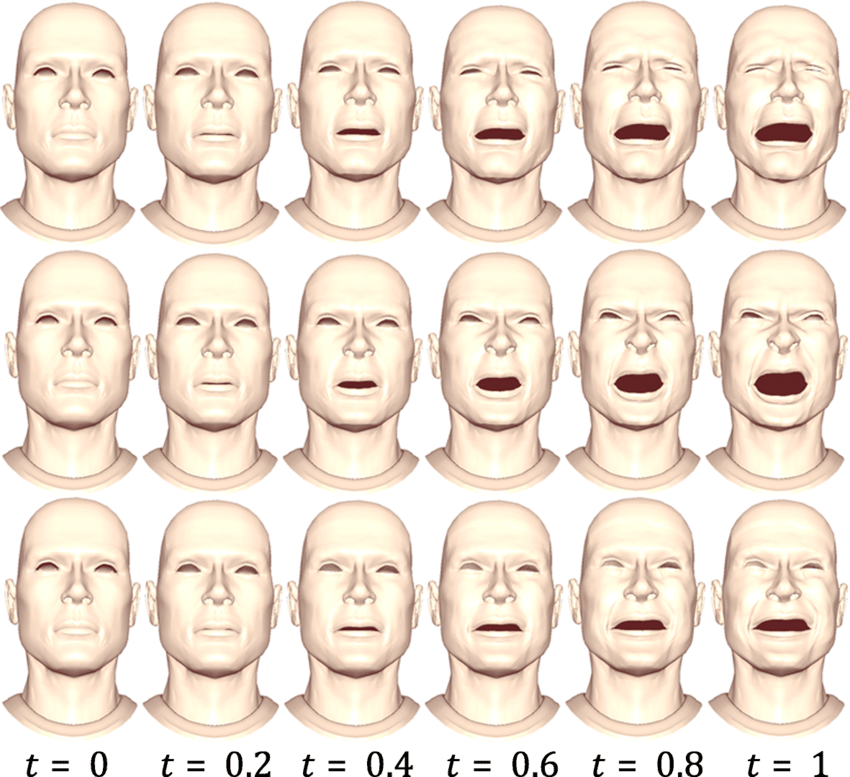
\includegraphics[width = 2.5in]{chapters/background_work/images/keyframing.png}
  \caption{Manual keyframing to animate an avatar}
  \label{fig:keyframing}
\end{figure}

Along with keyframing, motion curves\cite{0.1145/218380.218422} are used to control the interpolation between keyframes. These curves define the speed and timing of the animation, allowing animators to create smooth and natural movements. Common types of motion curves include linear, ease-in, ease-out, and bezier curves. By adjusting the shape and slope of these curves, animators can fine-tune the animation to achieve the desired effect\ref{fig:motion_curves}.

\begin{figure}
  \centering 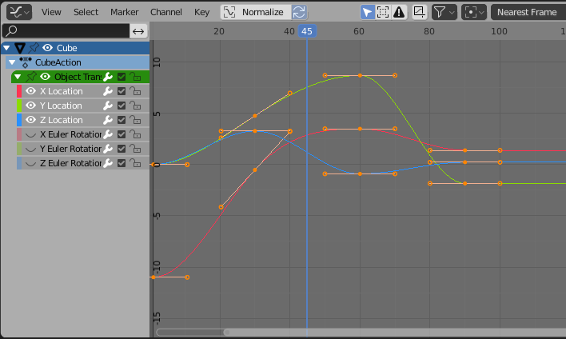
\includegraphics[width = 2.5in]{chapters/background_work/images/motion_curves.png}
  \caption{Motion curves to finetune an animation}
  \label{fig:motion_curves}
\end{figure}

\subsubsection{Mocap Retargeting}

Motion capture (mocap) retargeting involves capturing the movements of a real human actor and applying this data to a digital avatar. This process starts with recording an actor’s performance using a motion capture system, which tracks the actor’s movements through markers or sensors placed on their body \ref{fig:mocap}. The recorded data is then mapped onto the avatar’s skeleton, a process known as retargeting. Mocap retargeting ensures highly realistic animations by directly transferring the nuances of human motion to the digital character. This technique is widely used in the entertainment industry, particularly in video games and films, to create lifelike animations. While mocap retargeting can significantly speed up the animation process and improve realism, it requires access to specialized equipment and can involve complex data processing to filter noise.

\begin{figure}
  \centering 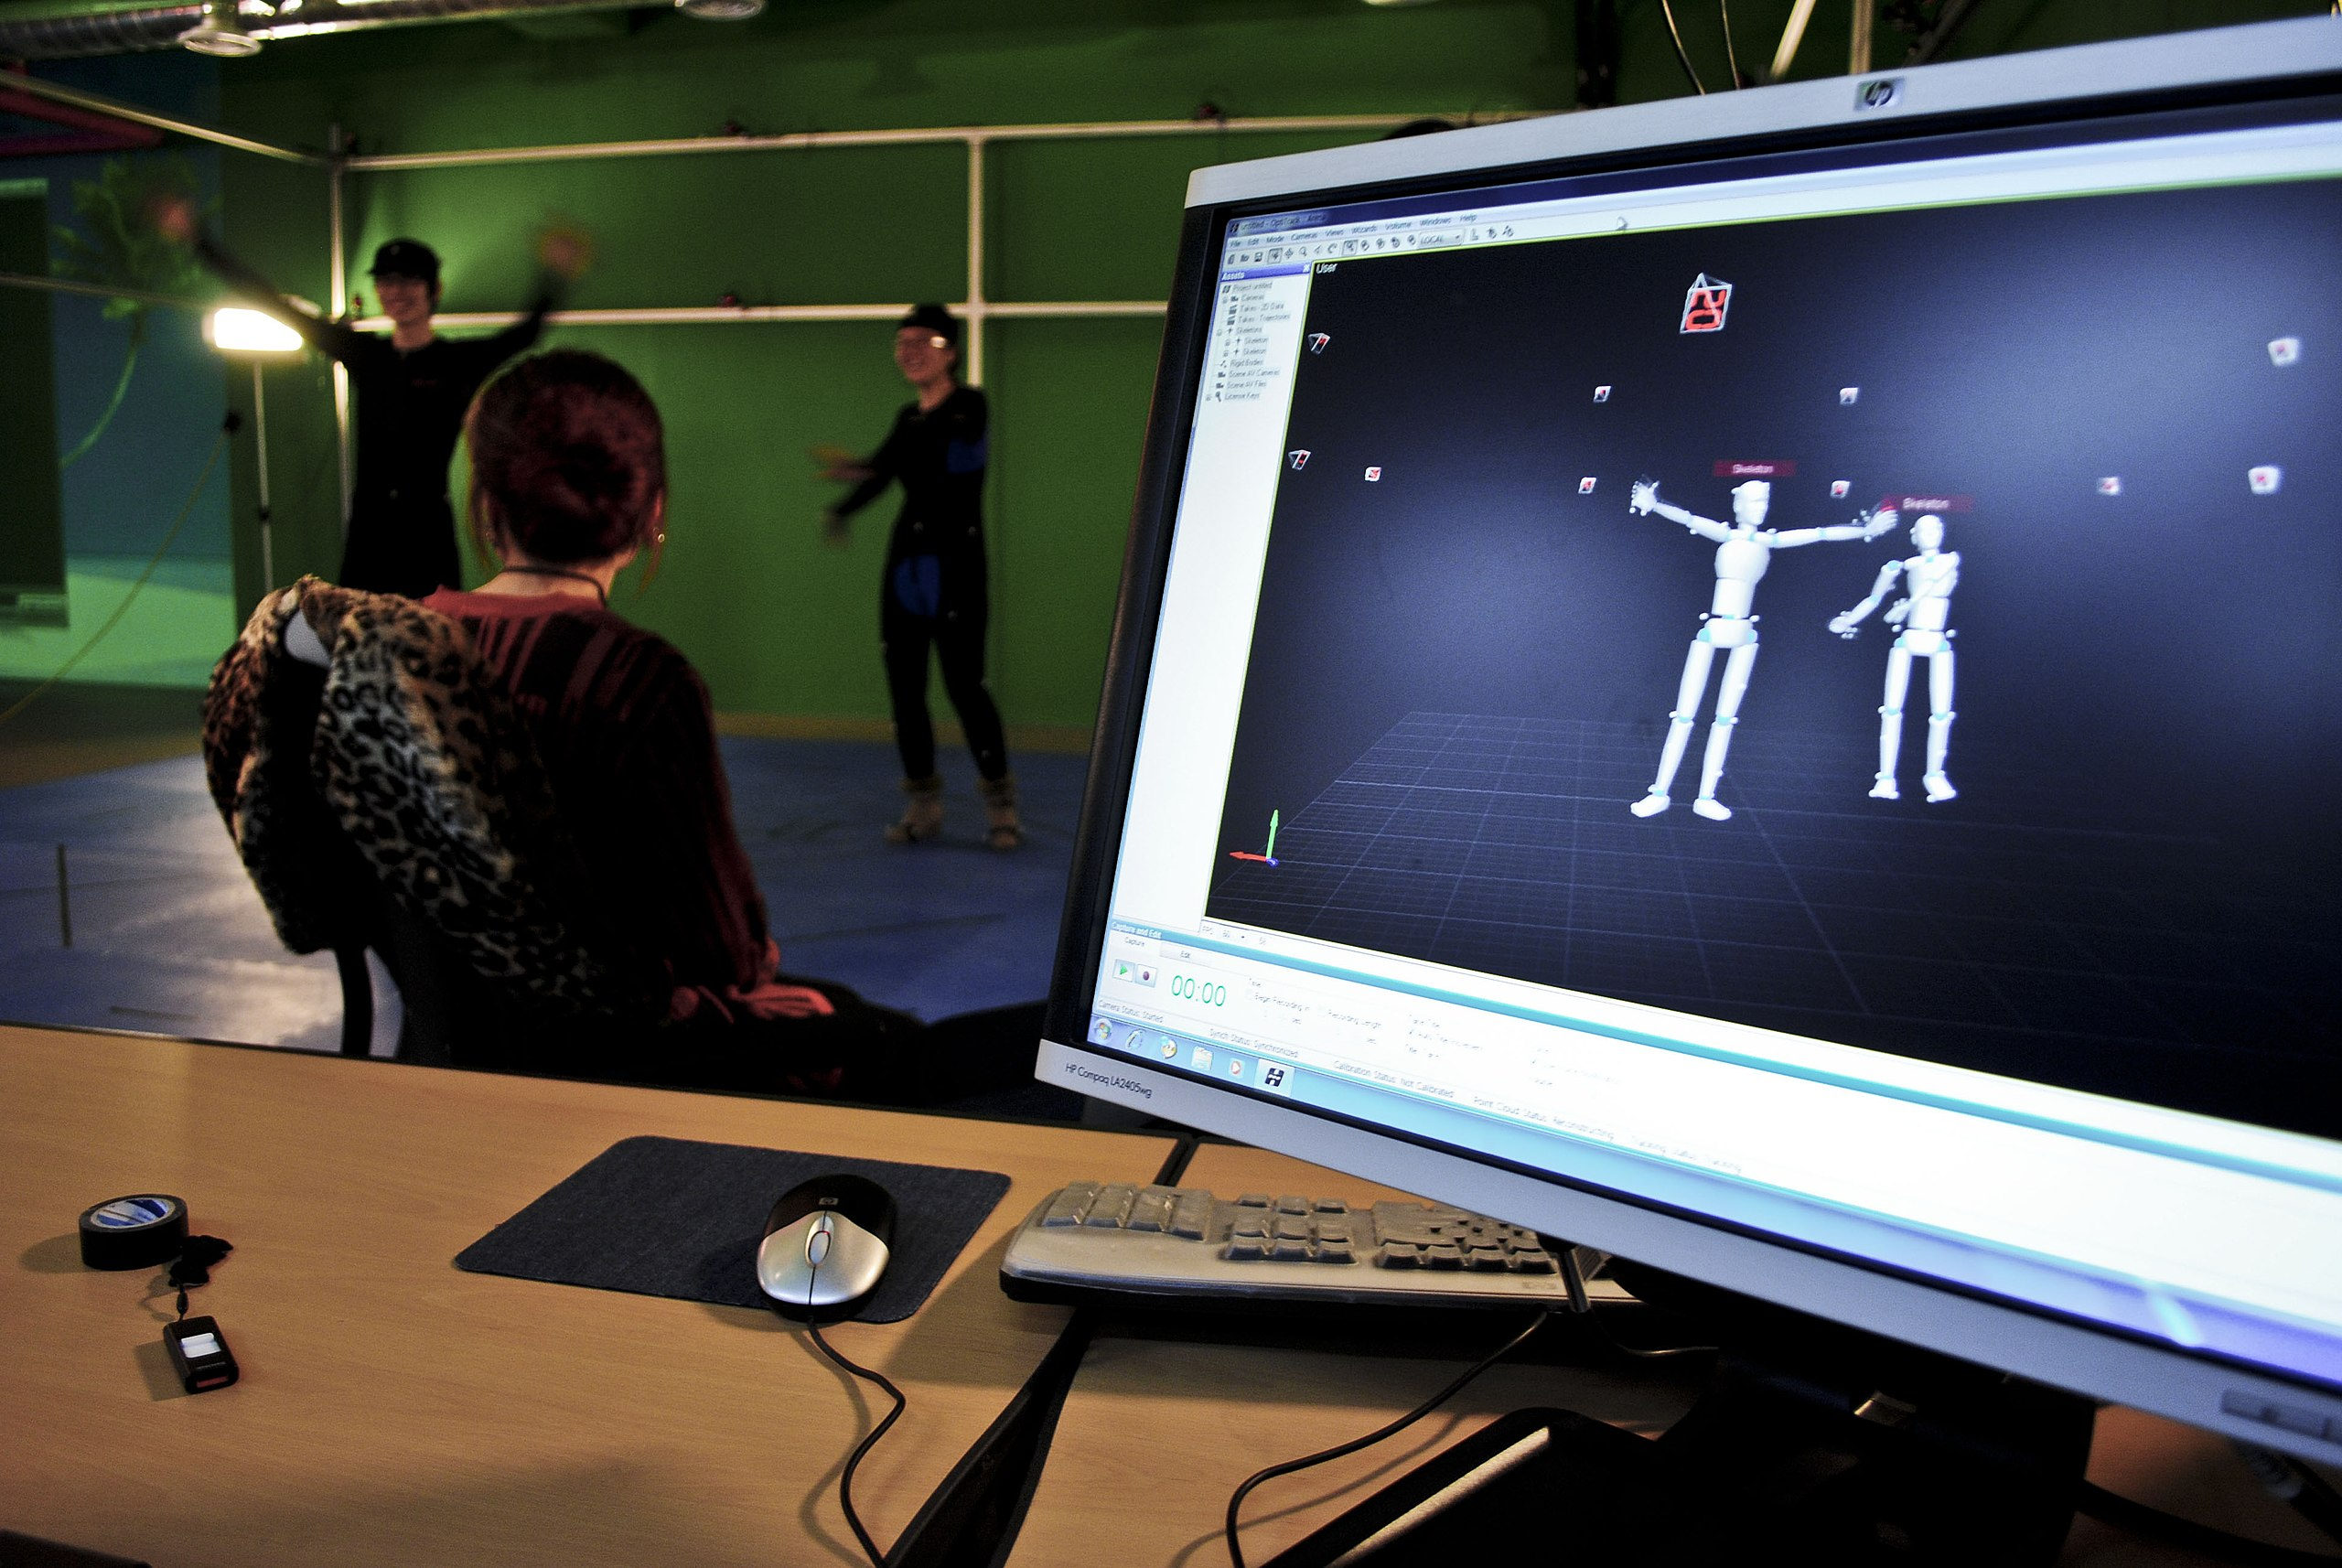
\includegraphics[width = 2.5in]{chapters/background_work/images/mocap.png}
  \caption{Mocap capture and retargeting}
  \label{fig:mocap}
\end{figure}

\subsubsection{Kinematics}

Kinematics is a subfield of physics and mathematics, developed in classical mechanics, that describes the motion of points, bodies (objects), and systems of bodies (groups of objects) without considering the forces that cause them to move. In context of avatar animation, kinematics is used to define the motion of joints in a skeleton, allowing animators to create realistic and dynamic movements. Two key kinematic techniques used in avatar animation are forward kinematics (FK) and inverse kinematics (IK).

\paragraph{Forward Kinematics}

Forward kinematics (FK) is a method where the position and rotation of each joint in a skeleton are specified explicitly by the animator. This means that to move a hand, for example, the animator must adjust the shoulder, elbow, and wrist joints individually. FK provides precise control over each joint, making it ideal for detailed and deliberate animations. However, it can be cumbersome for complex movements, as changes to one joint may require adjustments to multiple other joints to achieve a natural pose \ref{fig:forward_kinematics_example}.

\begin{figure}
  \centering 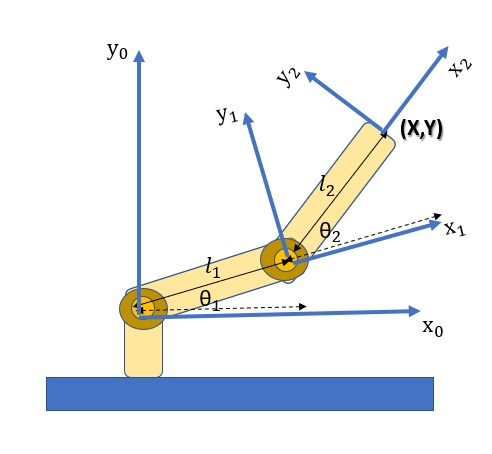
\includegraphics[width = 2.5in]{chapters/background_work/images/forward_kinematics_example.png}
  \caption{Forward kinematics}
  \label{fig:forward_kinematics_example}
\end{figure}

\paragraph{Inverse Kinematics}

Inverse kinematics (IK) simplifies the animation process by allowing the animator to position the end effector (e.g., a hand or foot) directly, and the software automatically calculates the necessary joint rotations to achieve this position\ref{fig:inverse_kinematics_example}. This technique is particularly useful for tasks like making a character’s hand reach a specific point or ensuring that feet remain planted on the ground. IK is widely used in character animation to create natural and realistic movements more efficiently than FK.

IK solvers are algorithms that compute the necessary joint rotations to achieve a desired position of the end effector. Different IK solvers are available, each with its unique approach and strengths. Here are a few popular IK solvers:

\begin{itemize}
  \item \textbf{iTaSc (Instantaneous Task Specification using Constraints)}: iTaSc\cite{4648032} operates by formulating the IK problem as a set of instantaneous task specifications, which are treated as constraints. These constraints can include positions, orientations, and other task-specific requirements. The method solves the IK problem by minimizing a cost function subject to these constraints. It utilizes optimization techniques to handle multiple, potentially conflicting constraints simultaneously, ensuring that the solution adheres to the defined task requirements.

  \item \textbf{CCDIK (Cyclic Coordinate Descent Inverse Kinematics)}: CCDIK\cite{kenwright2012inverse} works by iteratively optimizing the position of each joint in the kinematic chain. Starting from the end effector, the algorithm adjusts each joint to minimize the distance between the end effector and the target position. This is done in a cyclic manner, where each joint is adjusted in sequence until the end effector reaches an acceptable proximity to the target. The process is repeated iteratively, ensuring that the adjustments of one joint do not significantly disrupt the adjustments of previous joints.

  \item \textbf{FABRIK (Forward And Backward Reaching Inverse Kinematics)}: FABRIK\cite{aristidou2011fabrik} operates through a two-phase iterative process: forward reaching and backward reaching. In the forward reaching phase, the algorithm starts from the base of the kinematic chain and moves towards the end effector, adjusting each joint to align with the target position while respecting joint constraints. In the backward reaching phase, the algorithm starts from the end effector and moves back towards the base, further refining joint positions to ensure convergence towards the target. This alternating process continues until the end effector reaches the desired target within an acceptable tolerance.
\end{itemize}

\begin{figure}
  \centering 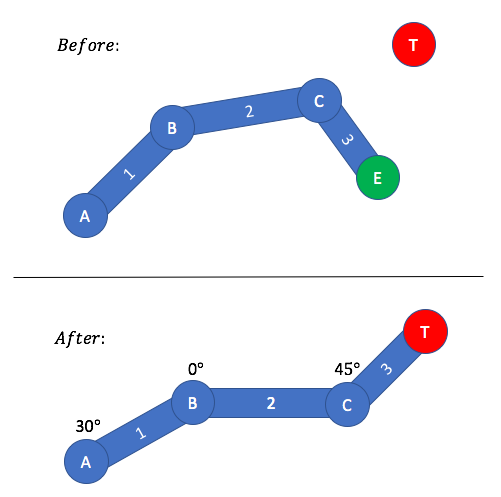
\includegraphics[width = 2.5in]{chapters/background_work/images/inverse_kinematics_example.png}
  \caption{Inverse kinematics}
  \label{fig:inverse_kinematics_example}
\end{figure}

\subsubsection{Procedural Techniques}

Procedural animation techniques use algorithms and rules to generate motion automatically, rather than relying on manual keyframing or motion capture data. These techniques are particularly useful for creating dynamic and responsive animations that adapt to changing conditions or user interactions. Procedural animation can be applied to various aspects of avatar animation, including locomotion, facial expressions, and secondary motion.


\paragraph{Data-Driven Constraint-Based Motion Editing}

Data-driven constraint-based motion editing\cite{inbook} combines model-based and goal-directed techniques to enhance human motion animation. The system incorporates Prioritized Inverse Kinematics (PIK) to solve for joint movements that meet user-defined constraints. Animators can use key-frame and key-trajectory constraints to specify end-effector positions and paths, simplifying the animation process. The optimization step ensures  smooth, continuous motions, avoiding common artifacts and preserving the natural flow of movement. 

\paragraph{Deep Learning based Techniques}

Deep learning-based techniques have shown significant promise in procedural animation, particularly in the generation of realistic and dynamic movements. Neural networks can be trained on large datasets of motion data to learn complex patterns and generate new animations\ref{fig:deep_learning_synthesis}. For example, diffusion models\cite{zhang2022motiondiffuse} have been used to synthesize human-like motion sequences with high fidelity and diversity from text prompts. Treating character animation as a cross-modal translation task where descriptive sentences serve as inputs to generate corresponding avatar animations. These techniques however require large amounts of data and computational resources to train effectively.

\begin{figure}
  \centering 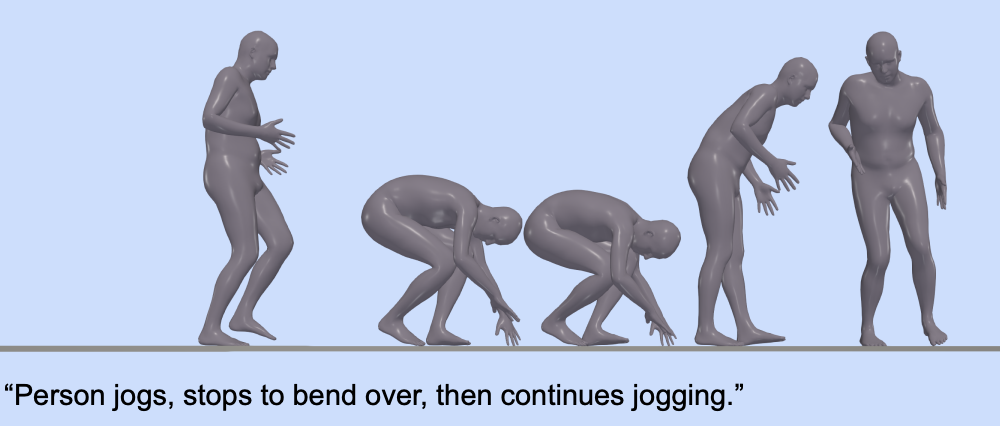
\includegraphics[width = 2.5in]{chapters/background_work/images/deep_learning_synthesis.png}
  \caption{Deep Learning based synthesis\cite{guo2022generating}}
  \label{fig:deep_learning_synthesis}
\end{figure}

\subsubsection{Hybrid}

Hybrid animation techniques combine elements of manual keyframing, mocap retargeting, and procedural techniques to leverage the strengths of each method. By integrating these approaches, animators can achieve a balance between control, efficiency, and realism. For instance, an animator might use mocap data as a base and then refine specific movements with manual keyframes to enhance expressiveness. Additionally, procedural techniques can be applied to automate repetitive tasks or to ensure that certain constraints are met dynamically during the animation process. Hybrid methods offer a flexible and powerful workflow, allowing for the creation of complex animations that are both realistic and tailored to the specific needs of a project\ref{fig:cascadeur}.

\begin{figure}
  \centering 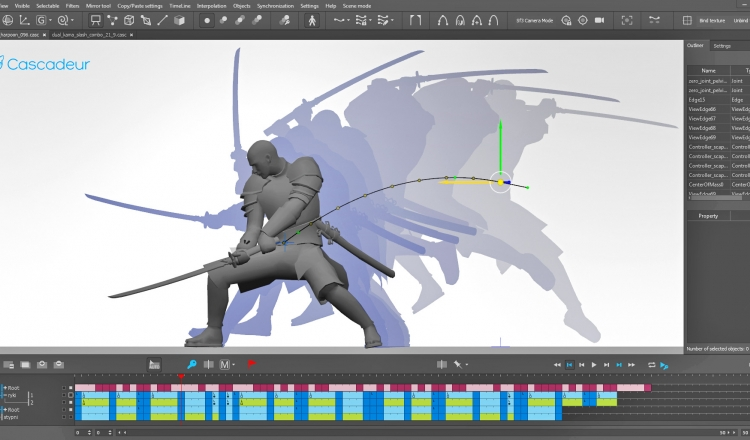
\includegraphics[width = 2.5in]{chapters/background_work/images/cascadeur.png}
  \caption{Cascadeur hybrid animation tool}
  \label{fig:cascadeur}
\end{figure}

\subsubsection{Uncanny Valley}

The Uncanny Valley is a concept in the field of robotics and 3D animation that describes the discomfort or eeriness that people experience when they encounter a humanoid figure that is very close to, but not quite, human-like. This phenomenon was first identified by roboticist Masahiro Mori in 1970.

As avatars become more realistic in appearance and movement, they initially become more appealing and relatable. However, there is a point at which the avatar becomes almost, but not perfectly, human-like, causing a sense of unease or revulsion in the observer. This dip in the graph of familiarity versus human likeness is known as the Uncanny Valley\ref{fig:uncanny_valley_graph}.

\begin{figure}
  \centering 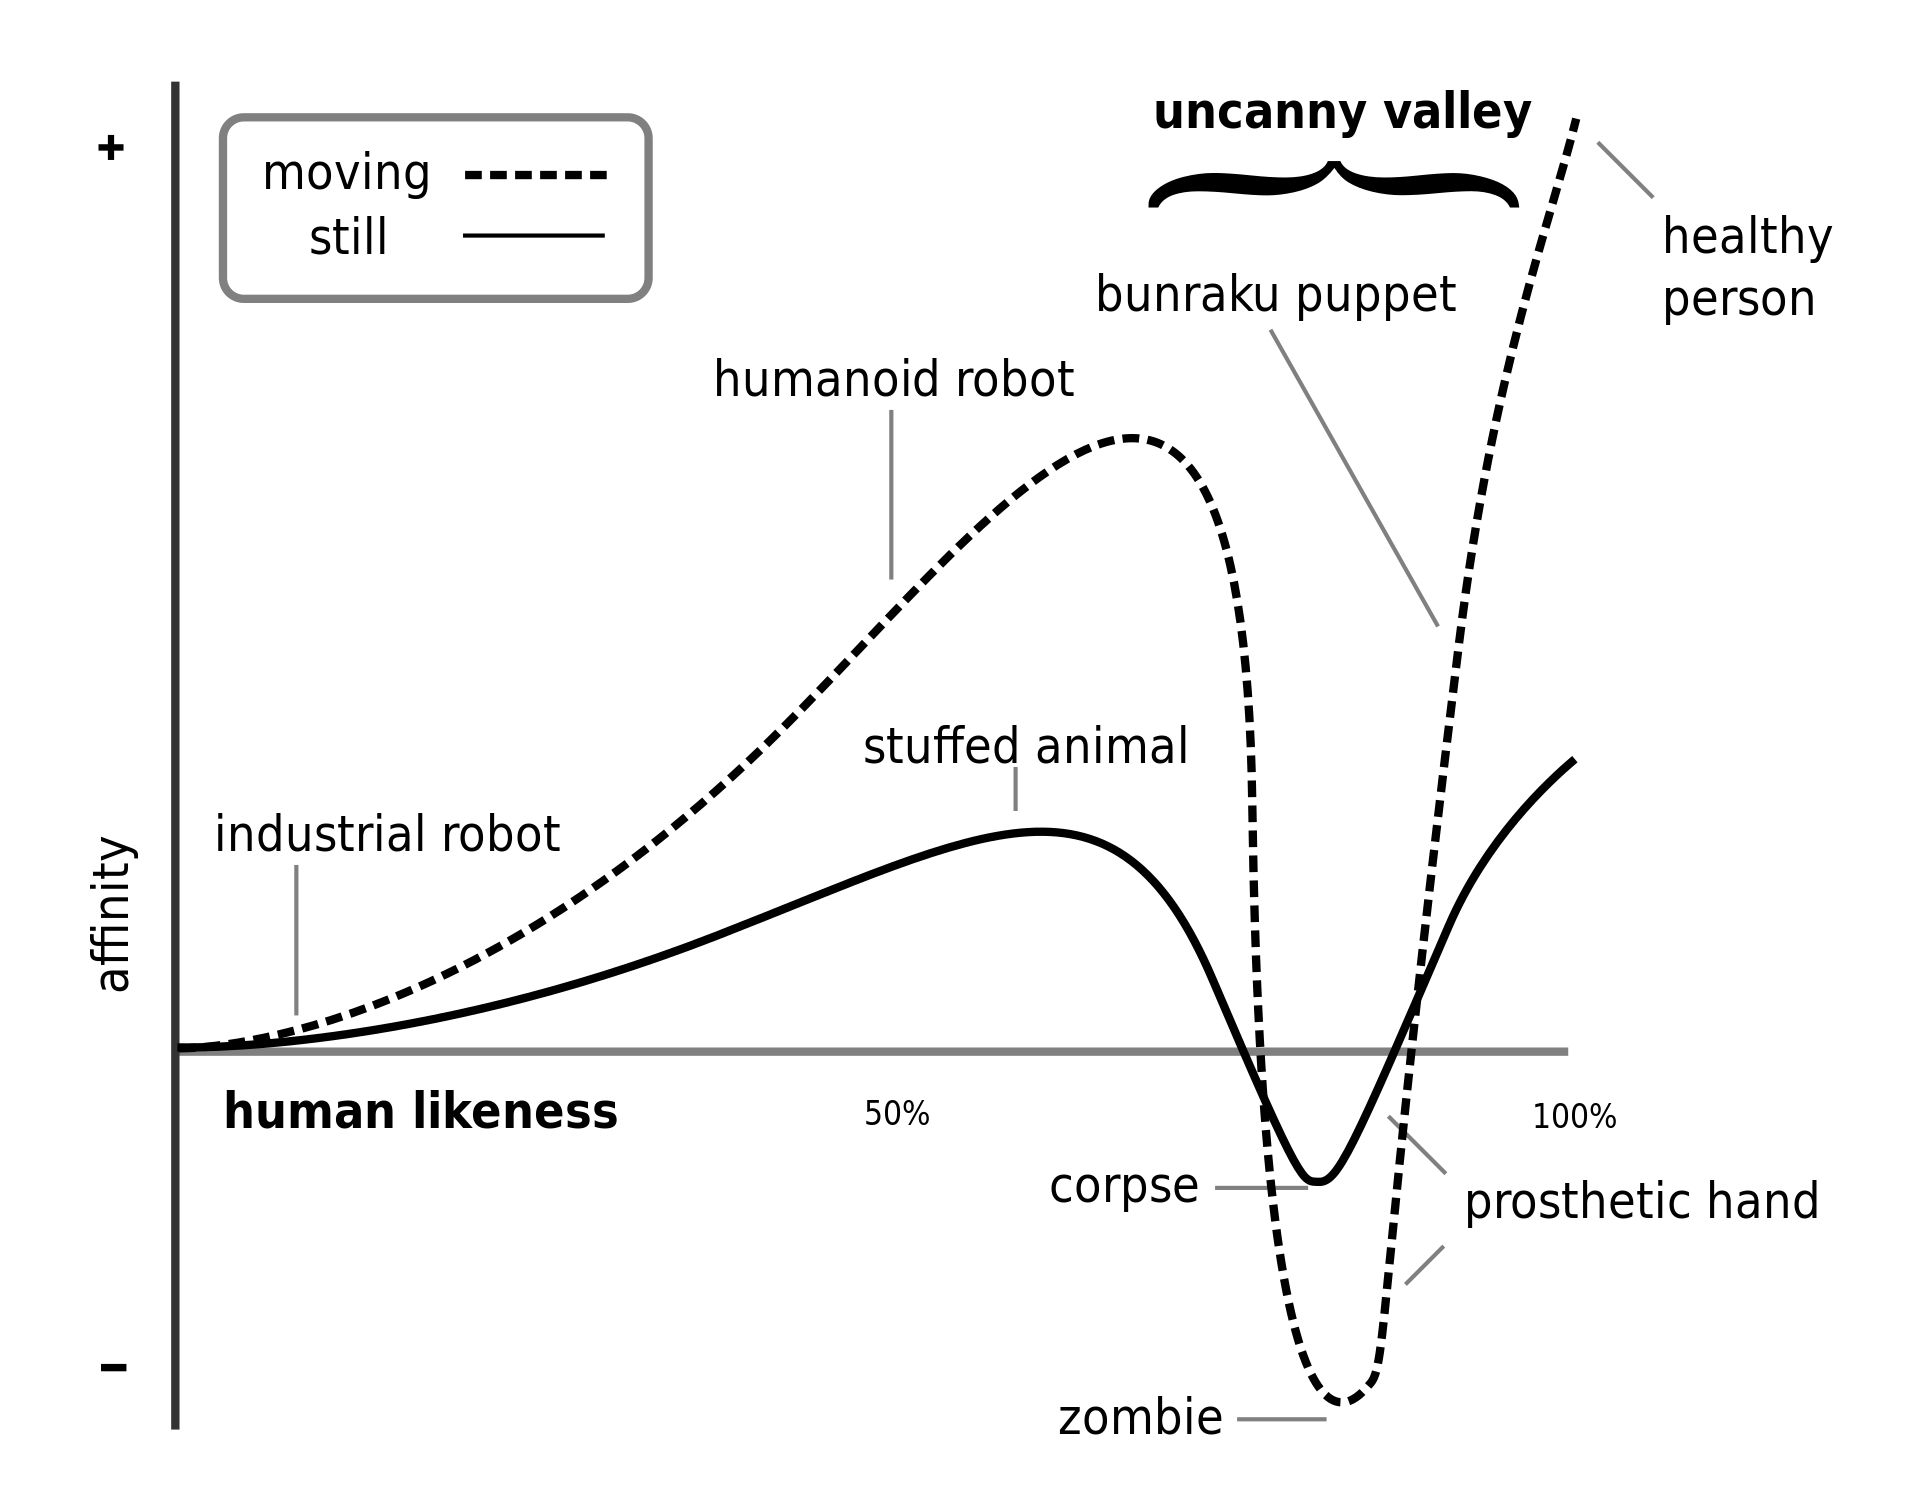
\includegraphics[width = 2.5in]{chapters/background_work/images/uncanny_valley_graph.png}
  \caption{Uncanny Valley}
  \label{fig:uncanny_valley_graph}
\end{figure}

The factors contributing to the Uncanny Valley effect often include:
\begin{itemize}
  \item \textbf{Facial Expressions}: Subtle imperfections in facial expressions, such as unnatural eye movements or lifeless smiles, can make the avatar appear creepy or unsettling.
  \item \textbf{Movement}: Non-human-like movements, jerky motions, or slight deviations from natural human motion can heighten the uncanny effect.
  \item \textbf{Texture and Skin Tone}: Inconsistent skin textures, overly smooth surfaces, or unrealistic lighting and shading can make an avatar appear artificial.
  \item \textbf{Eye Contact}: The eyes are critical in conveying emotions and life. Any deviation in eye movement, blink patterns, or focus can make an avatar look eerie.
\end{itemize}

Understanding and mitigating the Uncanny Valley effect is crucial for animators and developers aiming to create realistic and relatable avatars. One way to avoid uncanny valley could be to use stylized avatars, which are intentionally designed to deviate from realism and have a unique aesthetic\ref{fig:stylized_avatars}. Another way is to keyframe more information in the animations itself.

\section{Describing Sign Language}

A key challenge in Sign Language synthesis lies in the description of a Sign Language discourse itself. A description of a discourse can answer questions such as:

\begin{itemize}
  \item What body motions make a sign?
  \item How do these signs and their respective motions connect to form a discourse?
  \item What are the grammatical and syntactical rules governing these signs?
  \item How can non-manual signals (such as facial expressions and body posture) be integrated with manual signs?
  \item How can non-manual signals (such as facial expressions and body posture) be integrated with manual signs?
\end{itemize}

In this section, we first study the descriptive languages used to formalize sign languages and how they describe body motions.

Descriptive languages are systems developed to transcribe and analyze sign languages. They provide a framework for representing the complex, multi-dimensional nature of sign language communication. Some notable descriptive languages include:

\subsection{Lexical Descriptions}

Lexical descriptions focus on individual signs and their components, such as handshapes, movements, and locations. These descriptions are essential for understanding the building blocks of sign language and how signs are produced. Some popular lexical descriptions include:

\subsubsection{Stokoe Notation}

Stokoe Notation\cite{stokoe1980sign} was one of the first systems developed to transcribe American Sign Language (ASL). It breaks down signs into three main components: location, handshape, and movement\ref{fig:stoeke}. It is a simple and effective notation for basic transcription, but focuses primarily on the manual components of signs.

\begin{figure}
  \centering 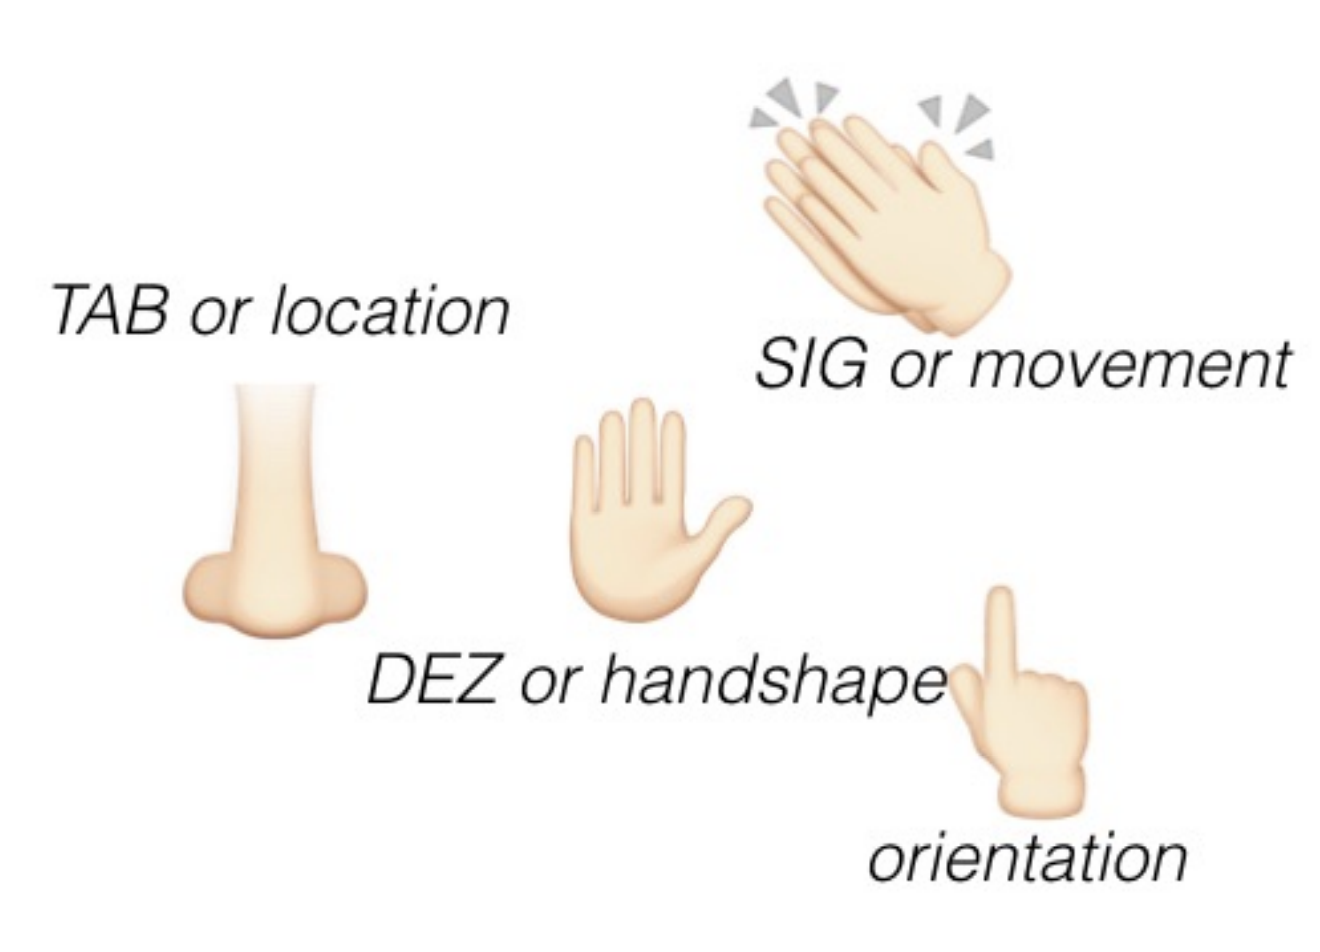
\includegraphics[width = 2.5in]{chapters/background_work/images/stokoe.png}
  \caption{Stoeke Notation}
  \label{fig:stoeke}
\end{figure}

\begin{figure}
  \centering 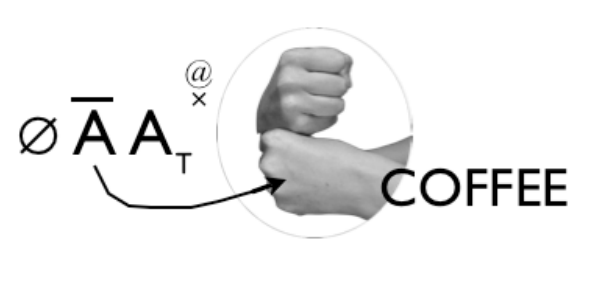
\includegraphics[width = 2.5in]{chapters/background_work/images/stokoe_coffee.png}
  \caption{Coffee in Stokoe Notation}
  \label{fig:stoeke_coffee}
\end{figure}

A lot of subsequent systems were discovered inspired by Stokoe's approach. These systems are more complex and detailed, and they aim to capture the nuances of sign language more accurately.

\subsubsection{SignWriting}

SignWriting is a writing system developed by Valerie Sutton just after DanceWriting\cite{sutton1973sutton} in the 1970s to represent sign languages visually. It was later included as a part of the MovementWriting system. It is a featural script, meaning that it represents the features of signs, such as handshapes, movements, and locations, rather than phonetic sounds. SignWriting is designed to be easy to read and write, with symbols that resemble the gestures they represent. The script is written in two dimensions, with symbols arranged in a grid-like structure to capture the spatial and temporal aspects of signs. SignWriting has been used to transcribe over 40 sign languages worldwide and is recognized by the International SignWriting Alphabet (ISWA) organization.

\begin{figure}
  \centering 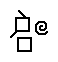
\includegraphics[width = 2.5in]{chapters/background_work/images/signwriting_coffee.png}
  \caption{Coffee in SignWriting}
  \label{fig:signwriting_coffee}
\end{figure}

\subsubsection{HamNoSys}

The Hamburg Sign Language Notation System (HamNoSys) is a phonetic transcription system for documenting sign languages globally, developed in 1985 at the University of Hamburg. Unlike Stokoe's notation, which was specifically created for American Sign Language (LSF), HamNoSys aims for broader application, transcending national sign language boundaries. While Stokoe notation later adapted to other sign languages, HamNoSys was designed from the outset to accommodate the diversity found in global sign languages.

The notation system includes nearly 200 symbols categorized into five main types, which together depict the parameters of a sign. These symbols can include subscripts, superscripts, and diacritics. A sign is described through a series of these symbols, listed in a specific order:

\begin{itemize}
    \item \textbf{Handshape}: Describes the hand configuration, including the number and position of extended fingers, degree of finger bending, and thumb location. Common symbols include ovals and lines to signify finger positions and curves to represent bending.
    \item \textbf{Hand Orientation}: Indicates the orientation of the hand and direction of the fingers or palm. Symbols include ovals with thick sides and small arrows or carets for advanced angles.
    \item \textbf{Hand Location}: Specifies where the hand is positioned relative to the body, using symbols that often resemble the body parts involved, with a black square marking the feature's orientation.
    \item \textbf{Movement (Optional)}: Details any motion in the sign, such as direction and type of movement (e.g., straight, wavy, circular). These are represented by complex symbols with arrows, lines, and brackets to show sequential or unified movements.
    \item \textbf{Symmetry Operator (Optional)}: Indicates if both hands are used or specifies the use of the non-dominant hand, usually represented by two dots.
    \item \textbf{Non-Manual Marker (NMM) (Optional)}: Denotes facial or vocal actions accompanying the sign, such as lip-pursing or eyebrow-raising.
\end{itemize}

HamNoSys offers a detailed representation of the nuanced components in sign language discourse rather than serving as a practical writing system. Its main purpose is linguistic, used primarily by linguists to analyze the specific features of individual signs. However, it has also found it's applications in synthesis\ref{elliott2010towards} as well has sign detection\ref{mocialov2022unsupervised}.

\begin{figure}
  \centering 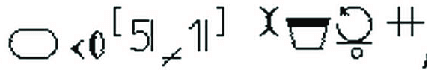
\includegraphics[width = 2.5in]{chapters/background_work/images/hamnosys_coffee.png}
  \caption{Coffee in HamNoSys}
  \label{fig:hamnosys_coffee}
\end{figure}

\subsection{Arranging Lexicals}

A sign language description is represented as an arrangement of lexicals or glosses. This arrangement can be sequential(linear) or non-linear.

\subsubsection{Sequential Arrangement}

Sequential arrangement of lexicals is a linear representation of sign language discourse. In this approach, signs are listed in the order they appear in the discourse, with each sign described using lexical notation. This method is straightforward and easy to follow, making it suitable for basic transcription and analysis. However, it may not capture the full complexity of sign language, particularly the non-linear aspects of signing such as simultaneous movements and facial expressions.

The following is an example of a sequential arrangement of lexicals for the sentence "I had coffee":
\begin{center}
  \textcolor{brown}{\textbf{COFFEE + I + HAD}}
\end{center}

\subsubsection{P/C Model}

Unlike HamNoSys, the Prosodic and Chronemic Model (P/C Model) \ref{huenerfauth2006generating} is a non-linear framework for describing sign language. This model focuses on capturing the rhythmic and temporal aspects of signing, recognizing that the timing and flow of signs are essential for their meaning. The P/C Model is particularly useful for understanding the nuances of sign language that go beyond simple hand movements, including the speed, intensity, and pauses that convey additional meaning. However, it has not been adopted for sign language synthesis.

\subsubsection{Canadian stuff}

https://github.com/PhonologicalCorpusTools try to define sign language phonology based on articulatory features but has no synthesis applications.

\subsubsection{AZee}

The AZee model is based on the notion of production rule, which associates a meaning to a set of observable forms. The model is based on the idea that the meaning of a sign can be decomposed into a set of features, which can be represented as a set of production rules. These rules are then used to generate the form of the sign, including the handshape, movement, and location. The AZee model is designed to be flexible and extensible, allowing for the representation of a wide range of signs and sign languages. It is particularly well-suited for sign language synthesis, as it provides a systematic and structured approach to describing signs and their components. Recently, it has also been extended to a writing system.

Examlple, the AZee visual description for a person aged 52 is shown in figure \ref{fig:azvd}. The corresponding AZee code for this would be:

:info-about
	'topic
	:une personne
	'info
	:info-about
		'topic
		:âge
		'info
		:tens-units
			'tens
			.nb-5
			'units
			.nb-2

\begin{figure}
  \centering 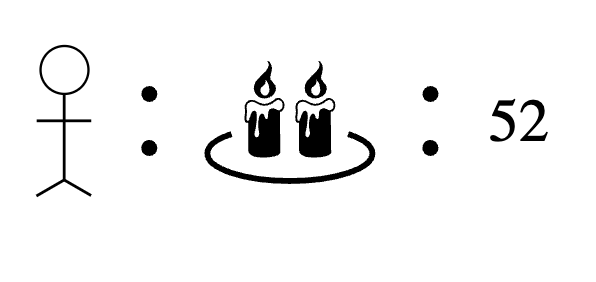
\includegraphics[width = 2.5in]{chapters/background_work/images/azvd.png}
  \caption{AZee visual description for a person aged 52}
  \label{fig:azvd}
\end{figure}

\section{Sign Language Synthesis}

Sign Language synthesis is the process of generating sign language animations from linguistic input. This process involves resolving a linguistic description into the anatomy of the avatar such as handshapes, movements, facial expressions, etc. on an avatar.  Sign Language synthesis is a complex and interdisciplinary field that draws on linguistics, computer science, animation, and human-computer interaction. Several approaches have been developed to synthesize sign language animations, each with its unique strengths and challenges.

\subsection{JASigning}

JASigning is an advanced sign language avatar system developed within the scope of the ViSiCAST and eSIGN projects\cite{elliott2010towards}. It enables the automatic generation and animation of sign language through a predefined set of gestures and animations. These gestures can be dynamically combined to form coherent sign language sentences. JASigning is designed to support multiple sign languages and integrates with text-to-sign translation systems. The system uses HamNoSys in the form of an XML representation\cite{elliott2004overview} to describe signs and their components. JASigning has been used in various applications, including educational tools, communication aids, and virtual avatars.

\begin{figure}
  \centering 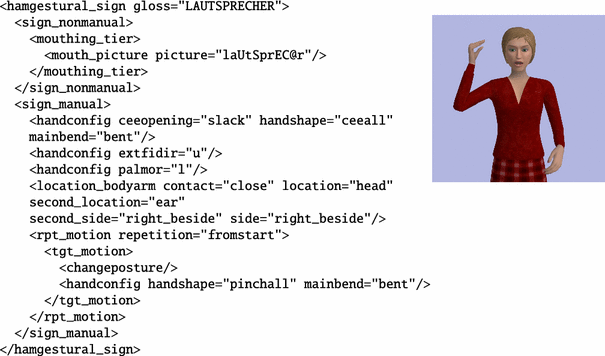
\includegraphics[width = 2.5in]{chapters/background_work/images/jasigning.png}
  \caption{JASigning}
  \label{fig:jasigning}
\end{figure}

\subsection{EMBR}

Unlike the previous models, EMBR (Embodied Agents Behaviour Realizer) Script \ref{heloir2009embr} is a scripting language used to control virtual characters in general and is not restricted to sign language avatars. However, EMBRScript allows for animation specification through a sequence of key poses, each defined at specific time points for a precise specification of body movements, facial expressions, and other actions. This also makes it usable to describe signs with synthesis using an avatar in mind.

EMBR (Embodied Agents Behaviour Realizer)\cite{heloir2010real} is a real-time animation engine engineered to produce expressive gestures and sign language for virtual avatars. EMBR facilitates precise control over avatar movements, encompassing hand shapes, facial expressions, and body postures critical for accurate sign language depiction. The framework supports scripting and integrates with various input modalities, such as text or motion capture data, to generate realistic and contextually appropriate sign language animations. EMBR's flexibility and adaptability make it a valuable tool in research settings, particularly for studies focused on the nuances of non-verbal communication and the development of nuanced, context-sensitive gestures.

\subsection{Sign3D}

The Sign3D project developed tools for high-fidelity 3D recording of French Sign Language (LSF) using an optical motion capture system with head-mounted oculometers. They annotated captured data with Elan software, segmenting signs and adding meta-data. A visual composition interface was created for assembling new sentences from the database. These motion capture chunks were concatenated and optimized for smooth transitions. The process concluded with rendering a 3D virtual signer for accurate motion playback.

\subsection{Synthesis based on generative models}

Generative models have shown promise in sign language synthesis by learning the underlying structure of sign language data and generating new animations. These models can be trained on large datasets of sign language videos to capture the complex relationships between linguistic input and sign language output. Some popular generative models used in sign language synthesis include:

\subsubsection{Gloss based}

Sign language animation from text focuses on generating realistic sign language videos from written text. The process involves text-to-gloss conversion, gloss-to-pose generation, and pose-to-sign rendering. Recent approaches utilize neural networks and generative models to enhance animation fluidity and realism. One method uses dictionary examples and a codebook of signs to create continuous sign language sequences, incorporating both manual and non-manual features\cite{Walsh2024ADR}. However, challenges remained in annotating the data and training the models effectively, particularly in the production of natural hand and facial movements.

\subsubsection{Sign Writing based}

Another approach\cite{jiang-etal-2023-machine} used the SignBank dataset, which contains 220k parallel samples of SignWriting and spoken language text. SignWriting served as an intermediate representation, translating spoken text into SignWriting before converting it into human poses\ref{fig:sw_synthesis}. Neural machine translation (NMT) architectures with techniques like byte pair encoding (BPE) segmentation were used. Evaluations show over 30 BLEU scores in bilingual settings and over 20 BLEU in multilingual settings, validating the approach and highlighting the effectiveness of SignWriting in NLP for sign language processing.

\begin{figure}
  \centering 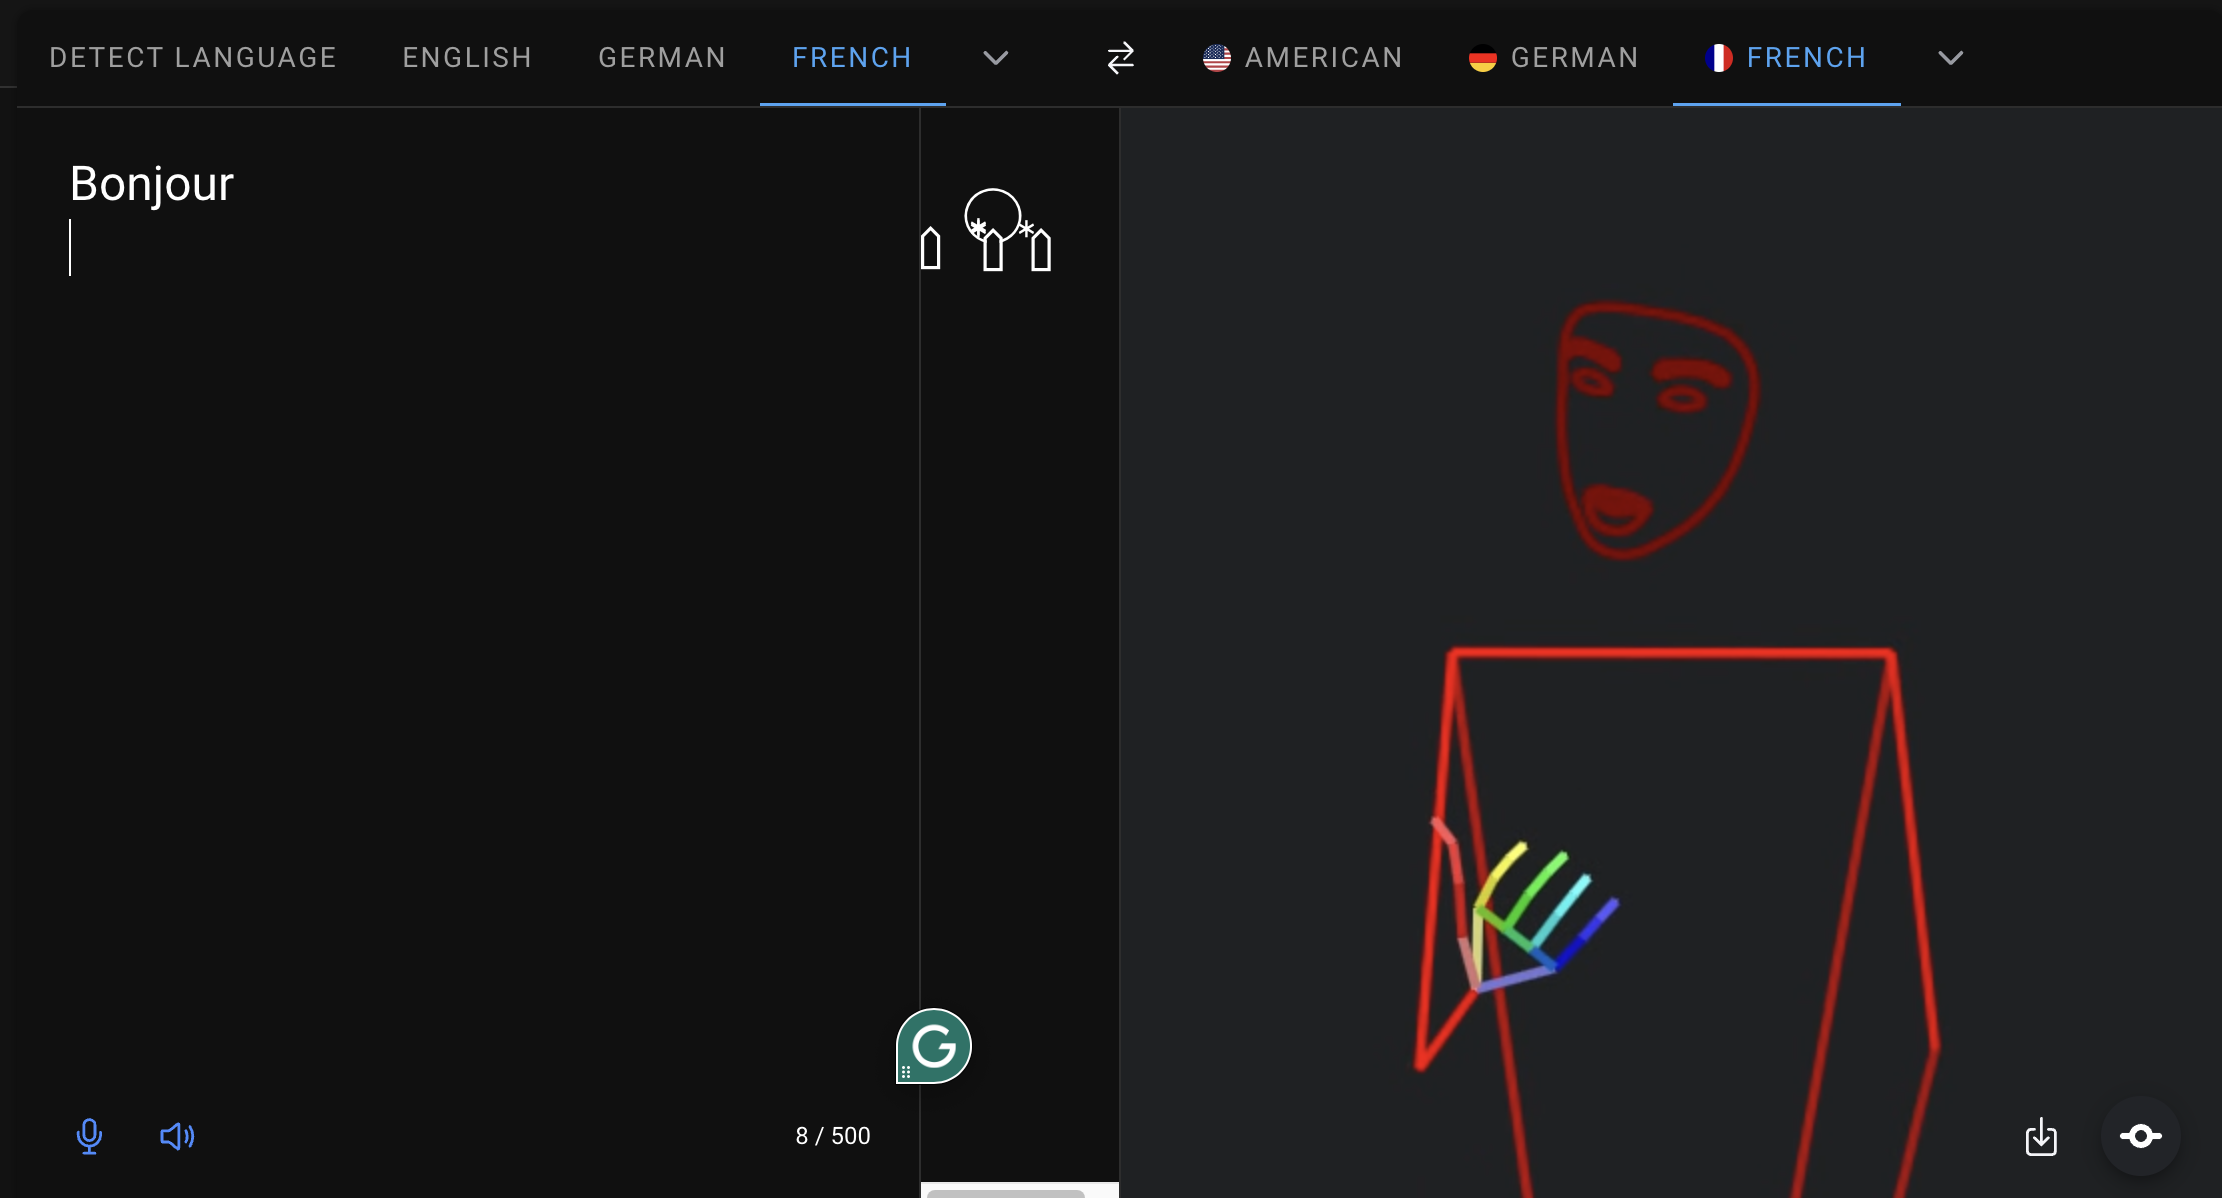
\includegraphics[width = 2.5in]{chapters/background_work/images/sign_writing_synthesis.png}
  \caption{Synthesis using SignWriting as an intermediate representation}
  \label{fig:sw_synthesis}
\end{figure}

\subsubsection{SignAvatars}

The SignAvatars dataset introduces a large-scale, multi-prompt 3D sign language motion dataset with 70,000 videos and 8.34 million frames from 153 signers. It includes isolated and continuous signs, annotated with 3D meshes and biomechanically-valid poses. The dataset supports tasks such as 3D sign language recognition and production from text scripts, individual words, and HamNoSys notation. A novel annotation pipeline ensures accurate 3D holistic annotations. Evaluation metrics indicate significant improvements in generating natural and consistent 3D sign language animations from diverse textual inputs using models like Sign-VQVAE.

\subsubsection{Sgnify}

Recent advancements in sign language processing involve synthesizing sign language animations from textual descriptions. The process includes text-to-gloss conversion, gloss-to-pose generation, and pose-to-sign rendering. One notable approach uses neural networks to convert text into SignWriting, which is then transformed into human poses. SGNify utilizes linguistic priors and SMPL-X for accurate 3D hand pose, facial motion, and body pose from monocular video. Techniques such as filtering in the frequency domain and resampling ensure natural rhythm and prosody, overcoming challenges like motion blur and occlusion, resulting in more comprehensible and natural sign language animations.

\subsection{AZee based}

\subsubsection{Paula}

The system extends the Paula\cite{azee-paula} avatar using AZee descriptions. AZee encodes both form and functional linguistic aspects, while Paula ensures smooth human motion. The approach leverages a hierarchical model to specify movements using larger linguistic structures, improving naturalness. Key innovations include embedding geometric constraints and utilizing procedural techniques for dynamic, realistic animations. Proform placements are optimized by factoring semantic functions and applying common forms across multiple productions. This method addresses limitations in previous models, such as the lack of supporting torso motion and dynamic differences, leading to more fluid and expressive sign language animations.\ref{mcdonald2016automated}

\subsubsection{Low-level synthesizor for AZee}

This work presents a bottom-up(or low-level generation using constraint optimization) synthesis solution for the AZee system using off-the-shelf IK solvers. The approach generates procedurally computed animations from AZee's symbolic descriptions, leveraging Blender's 3D editor and iTaSC solver. This method handles constraints as IK problems, translating skeletal poses into keyframes. Despite inherently robotic motion, it serves as a low-level fallback for the existing top-down system. Preliminary results show effective static pose generation and a trade-off between precision and computation time, enhancing the flexibility of sign language avatar systems by integrating procedural synthesis with predefined animations.\ref{nunnari2018animating}

\section{Conclusion}

To summarize:
\begin{itemize}
  \item Linear systems for sign language representation are limited in their expressive capacity and fail to capture the complexity of natural sign language.
  \item Non-linear systems provide better coverage and more accurately reflect the nuances of sign language.
  \item Systems like Paula and AZee, which incorporate both form and functional aspects, offer a promising approach but are hindered by the labor-intensive nature of hand-crafted animations.
  \item There is a need for low-level synthesis techniques to complement these high-level models, allowing for greater flexibility and coverage.
  \item Existing low-level synthesis approaches, such as those using IK solvers, provide a foundation but require further development to fully support the diverse requirements of sign language animation.
  \item By addressing these gaps, we aim to advance the state of sign language synthesis, making it more scalable and capable of generating natural and expressive animations.
\end{itemize}

Throughout this chapter, we have introduced, defined, and discussed a variety of concepts from three research areas that are key to this thesis: \textit{avatars}, \textit{sign language representation}, and \textit{sign language synthesis}. In the rest of the manuscript, we heavily rely on many of these concepts to investigate ways in which models for sign language synthesis can progressively learn and improve using newer techniques.

Therefore, in Chapter \ref{ch:multi-track} and Chapter \ref{ch:avatar_skeletal_layers}, we study and exploit multi-track representation and avatar layers for better discourses in sign language synthesis. Additionally, the studies presented in Chapter \ref{ch:intermediate_blocks}, Chapter \ref{ch:motiom_matching}, and Chapter \ref{ch:facial_expressions} dive deeper into reusing animations using a top-down search as they were described earlier in this chapter.

The background work specific to the various tasks and applications we address throughout the manuscript is presented and discussed in the corresponding chapters

\bibliography{background_work}
\end{document}